\documentclass[11pt,]{article}
\usepackage{lmodern}
\usepackage{amssymb,amsmath}
\usepackage{ifxetex,ifluatex}
\usepackage{fixltx2e} % provides \textsubscript
\ifnum 0\ifxetex 1\fi\ifluatex 1\fi=0 % if pdftex
  \usepackage[T1]{fontenc}
  \usepackage[utf8]{inputenc}
\else % if luatex or xelatex
  \ifxetex
    \usepackage{mathspec}
  \else
    \usepackage{fontspec}
  \fi
  \defaultfontfeatures{Ligatures=TeX,Scale=MatchLowercase}
\fi
% use upquote if available, for straight quotes in verbatim environments
\IfFileExists{upquote.sty}{\usepackage{upquote}}{}
% use microtype if available
\IfFileExists{microtype.sty}{%
\usepackage{microtype}
\UseMicrotypeSet[protrusion]{basicmath} % disable protrusion for tt fonts
}{}
\usepackage[margin=1.0in]{geometry}
\usepackage{hyperref}
\hypersetup{unicode=true,
            pdfborder={0 0 0},
            breaklinks=true}
\urlstyle{same}  % don't use monospace font for urls
\usepackage{graphicx,grffile}
\makeatletter
\def\maxwidth{\ifdim\Gin@nat@width>\linewidth\linewidth\else\Gin@nat@width\fi}
\def\maxheight{\ifdim\Gin@nat@height>\textheight\textheight\else\Gin@nat@height\fi}
\makeatother
% Scale images if necessary, so that they will not overflow the page
% margins by default, and it is still possible to overwrite the defaults
% using explicit options in \includegraphics[width, height, ...]{}
\setkeys{Gin}{width=\maxwidth,height=\maxheight,keepaspectratio}
\IfFileExists{parskip.sty}{%
\usepackage{parskip}
}{% else
\setlength{\parindent}{0pt}
\setlength{\parskip}{6pt plus 2pt minus 1pt}
}
\setlength{\emergencystretch}{3em}  % prevent overfull lines
\providecommand{\tightlist}{%
  \setlength{\itemsep}{0pt}\setlength{\parskip}{0pt}}
\setcounter{secnumdepth}{0}
% Redefines (sub)paragraphs to behave more like sections
\ifx\paragraph\undefined\else
\let\oldparagraph\paragraph
\renewcommand{\paragraph}[1]{\oldparagraph{#1}\mbox{}}
\fi
\ifx\subparagraph\undefined\else
\let\oldsubparagraph\subparagraph
\renewcommand{\subparagraph}[1]{\oldsubparagraph{#1}\mbox{}}
\fi

%%% Use protect on footnotes to avoid problems with footnotes in titles
\let\rmarkdownfootnote\footnote%
\def\footnote{\protect\rmarkdownfootnote}

%%% Change title format to be more compact
\usepackage{titling}

% Create subtitle command for use in maketitle
\newcommand{\subtitle}[1]{
  \posttitle{
    \begin{center}\large#1\end{center}
    }
}

\setlength{\droptitle}{-2em}

  \title{}
    \pretitle{\vspace{\droptitle}}
  \posttitle{}
    \author{}
    \preauthor{}\postauthor{}
    \date{}
    \predate{}\postdate{}
  
\usepackage{helvet} % Helvetica font
\renewcommand*\familydefault{\sfdefault} % Use the sans serif version of the font
\usepackage[T1]{fontenc}

\usepackage[none]{hyphenat}

\usepackage{setspace}
\doublespacing
\setlength{\parskip}{1em}

\usepackage{lineno}

\usepackage{pdfpages}

\begin{document}

\vspace{35mm}

\section{\texorpdfstring{Initial gut microbiota and response to
antibiotic perturbation influence \emph{Clostridioides difficile}
colonization in
mice}{Initial gut microbiota and response to antibiotic perturbation influence Clostridioides difficile colonization in mice}}\label{initial-gut-microbiota-and-response-to-antibiotic-perturbation-influence-clostridioides-difficile-colonization-in-mice}

\vspace{35mm}

Sarah Tomkovich\({^1}\), Joshua M.A.~Stough\({^1}\), Lucas
Bishop\({^1}\), Patrick D. Schloss\textsuperscript{1\(\dagger\)}

\vspace{40mm}

\(\dagger\) To whom correspondence should be addressed:
\href{mailto:pschloss@umich.edu}{\nolinkurl{pschloss@umich.edu}}

\(1\) Department of Microbiology and Immunology, University of Michigan,
Ann Arbor, MI 48109

\newpage

\linenumbers

\subsection{Abstract}\label{abstract}

The microbiota plays a key role in determining susceptibility to
\emph{Clostridioides difficile} infections (CDIs). However, much of the
mechanistic work examining CDIs in mouse models use a single university
colony or vendor. We treated mice from 6 different colony sources (2
University of Michigan colonies and 4 vendors) with a single clindamycin
dose, followed by \emph{C. difficile} challenge 1 day later and measured
\emph{C. difficile} colonization levels through 9 days post-infection.
The microbiota was profiled via 16S rRNA gene sequencing analysis to
examine variation across colony sources and alterations due to
clindamycin treatment and \emph{C. difficile} challenge. While all
sources of mice were colonized 1-day post-infection, variation in
\emph{C. difficile} colonization levels emerged from days 3-7
post-infection with 3 sources colonized with \emph{C. difficile} for
slightly longer and at higher levels. We identified bacterial taxa with
different relative abundances across colony sources throughout the
experiment, as well as taxa that were consistently impacted by
clindamycin treatment in all sources of mice. We created logistic
regression models that successfully classified mice based on whether
they cleared \emph{C. difficile} by 7 days post-infection using
baseline, post-clindamycin, and post-infection community composition
data. After examining the taxa that were most important to the
classification models, we identified a subset of key taxa that varied
across colony sources (\emph{Bacteroides}, \emph{Deferribacteraceae}),
were altered by clindamycin (\emph{Porphyromonadaceae},
\emph{Ruminococcaceae}), or both (\emph{Enterobacteriaceae},
\emph{Enterococcus}, \emph{Bifidobacteriaceae},
\emph{Coriobacteriaceae}, \emph{Lachnospiraceae}, and
\emph{Verrucomicrobiaceae}). These results suggest the response of the
initial gut microbiota to clindamycin treatment influences \emph{C.
difficile} 630 colonization dynamics.

\subsection{Importance}\label{importance}

\emph{Clostridioides difficile} is a leading nosocomial infection.
Although the microbiota has been established as a key risk factor, there
is variation in who becomes asymptomatically colonized, develops an
infection, or has an infection with adverse outcomes. \emph{C.
difficile} infection (CDI) mouse models are widely used to answer a
variety of \emph{C. difficile} pathogenesis questions. However, the
inter-individual variation between mice is less than what is observed in
humans, particularly if just one source of mice is used. In this study,
we administered clindamycin to mice from 6 different colony sources and
challenged them with \emph{C. difficile}. Interestingly, only a subset
of the taxa that vary across sources were associated with how long
\emph{C. difficile} was able to colonize. Future studies examining the
interplay between the microbiota and \emph{C. difficile} should consider
using mice from multiple sources to narrow down the microbes driving the
observed phenotypes and reflect human interindividual variation.

\newpage

\subsection{Introduction}\label{introduction}

Antibiotics are a clear risk factor for \emph{Clostridioides difficile}
infections (CDIs), but there is variation in who goes on to develop
severe or recurrent CDIs after exposure (1, 2). Additionally,
asymptomatic colonization, where \emph{C. difficile} is detectable, but
symptoms are absent has been documented in infants and adults (3, 4).
The intestinal microbiome has been implicated in asymptomatic
colonization (5, 6), susceptibility to CDIs (7), and adverse CDI
outcomes (9--12).

Mouse models of CDIs have been a great tool for understanding \emph{C.
difficile} pathogenesis (13). The number of CDI mouse model studies has
grown substantially since Chen et al. published their C57BL/6 model in
2008, which disrupted the gut microbiota with antibiotics to enable
\emph{C. difficile} colonization and symptoms such as diarrhea and
weight loss (14). CDI mouse models have been used to examine
translationally relevant questions regarding \emph{C. difficile},
including the role of the microbiota and efficacy of potential
therapeutics for treating CDIs (15). However, microbiome variation
between lab mice is much less than the variation observed between humans
(16, 17). Additionally, studying the contribution of the microbiota to a
particular disease phenotype in one set of lab mice after the same
perturbation could yield a number of findings of which only a fraction
may be driving the phenotype.

In the past, our group has attempted to introduce more microbiome
variation into the CDI mouse model by using a variety of antibiotic
treatments (18--21). An alternative approach to maximize microbiome
variation is to use mice from multiple sources (22, 23). Microbiome
differences between different mouse vendors have been well documented
and shown to influence susceptibility to a variety of diseases (24, 25),
including enteric infections (22, 23, 26--30). Additionally, different
research groups have observed different CDI outcomes in mice despite
using similar models and the microbiome has been proposed as one factor
potentially mediating susceptibility (13, 18, 21, 31--33). Here we
examined how variations in the baseline microbiome and responses to
clindamycin treatment in C57BL/6 mice from six different sources
influenced susceptibility to \emph{C. difficile} colonization and the
time needed to clear the infection.

\subsection{Results}\label{results}

\textbf{Clindamycin treatment renders all mice susceptible to \emph{C.
difficile} 630 colonization regardless of colony source.} To test how
the microbiotas of mice from different colony sources impact
colonization dynamics after clindamycin exposure, we utilized C57BL/6
mice from 6 different sources: two colonies from the University of
Michigan (the Young and Schloss lab colonies), the Jackson Laboratory,
Charles River Laboratories, Taconic Biosciences, and Envigo (which was
formerly Harlan). These 4 vendors were chosen because they represent
commonly used vendors for CDI studies in mice (26, 34--40). After a
13-day acclimation period for the mice ordered from vendors, all mice
were treated with 10 mg/kg clindamycin via intraperitoneal injection and
one day later challenged with 10\textsuperscript{3} \emph{C. difficile}
630 spores (Fig. 1A). Clindamycin was chosen because we have previously
demonstrated mice are rendered susceptible, but consistently cleared the
CDI within 9 days (21, 41), clindamycin is frequently implicated with
human CDIs (42), and is also part of the antibiotic treatment for the
frequently cited 2008 CDI mouse model (14). The day after infection,
\emph{C. difficile} was detectable in all mice at a similar level
(median CFU range: 2.2e+07-1.3e+08; \emph{P}\textsubscript{FDR} = 0.15),
indicating clindamycin rendered all mice susceptible regardless of
colony source (Fig. 1B). Interestingly, variation in \emph{C. difficile}
CFU levels across sources of mice emerged from days 3-7 post-infection
(all \emph{P}\textsubscript{FDR} \(\le\) 0.019; Fig. 1B and Table S1),
suggesting mouse colony source is associated with \emph{C. difficile}
clearance. We conducted two experiments approximately 3 months apart and
while the colonization dynamics were similar across most sources of
mice, there was some variation between the 2 experiments, particularly
for the Schloss and Envigo mice (Fig. S1A-B, Fig. 1D). Although \emph{C.
difficile} 630 causes mild symptoms in mice comparied to other \emph{C.
difficile} strains (43), we also saw that weight change significantly
varied across sources of mice with the most weight lost two days
post-infection (Fig. 1C, E and Table S2). Interestingly, mice ordered
from Jackson, Taconic, and Envigo tended to lose more weight (although
there was variation between experiments with Schloss and Envigo mice),
have higher \emph{C. difficile} CFU levels and take longer to clear the
infection compared to the other sources of mice, which was particularly
evident 7 days post-infection (Fig. 1B-E), when 57.50 of the mice were
still colonized with \emph{C. difficile} (Fig. S1C). By 9 days
post-infection the majority of the mice from all sources had cleared
\emph{C. difficile} (Fig. S1C) with the exception of 1 Taconic mouse
from the first experiment and 2 Envigo mice from the second experiment.
Importantly, there was also one Jackson and one Envigo mouse that died
between 1- and 3-days post-infection during the second experiment. Thus,
clindamycin rendered all mice susceptible to \emph{C. difficile} 630
colonization, regardless of colony source, but variation across sources
emerged with 3 out of 6 sources taking longer to clear \emph{C.
difficile}.

\textbf{Bacterial communities consistently vary across mouse colony
sources despite antibiotic and infection perturbations.} Given the well
known variation in mouse microbiomes across vendors and university
colonies (25), we hypothesized that the variation in \emph{C. difficile}
clearance could be explained by microbiota variation across the 6
sources. We used 16S rRNA gene sequencing to characterize the fecal
bacterial communities from the mice over the course of the experiment.
Since antibiotics and other risk factors of CDIs are associated with
decreased microbiota diversity (44), we first examined alpha diversity
measures across the 6 sources of mice. Examining the bacterial
communities at baseline, prior to clindamycin treatment there was a
significant difference in the number of observed OTUs
(\emph{P}\textsubscript{FDR} = 0.03), but not Shannon diversity index
(\emph{P}\textsubscript{FDR} = 0.052) across sources of mice (Fig. 2A-B
and Table S3). As expected, clindamycin treatment decreased richness and
Shannon diversity across all sources of mice, and communities started to
recover 1 day post-infection (Fig. 2C-D). Interestingly, significant
differences in diversity metrics across sources
(\emph{P}\textsubscript{FDR} \textless{} 0.05) emerged after both
clindamycin and \emph{C. difficile} infection, with Charles River mice
having higher richness and Shannon Diversity than most of the other
groups (Fig 2C-F and Table S4). While Charles River mice had more
diverse microbiotas, Young and Schloss lab mice were also able to clear
\emph{C. difficile} faster, suggesting microbiota diversity alone does
not explain the observed variation in \emph{C. difficile} colonization
across vendors.

Next, we compared the bacterial communities from the 6 colonies over the
course of the experiment using principal coordinate analysis (PCoA) of
the Theta YC distances. Permutational multivariate analysis of variance
(PERMANOVA) analysis revealed colony source was the major factor
explaining the observed variation across fecal communities
(R\textsuperscript{2} = 0.35, \emph{P} = 0.0001) followed by
interactions between cage and day of the experiment (Movie S1 and Table
S5). Since, the majority of the perturbations happened over the initial
days of the experiment, we decided to focus on the bacterial communities
at baseline (day -1), after clindamycin treatment (day 0), and
post-infection (day 1). For all 3 timepoints, source and the interaction
with cage significantly explained most of the observed community
variation (combined R\textsuperscript{2} = 0.90, 0.99, 0.88,
respectively; \emph{P} = 0.0001; Fig. 3 and Table S6). We also compared
baseline communities across the 2 experiments, and found experiment and
cage significantly explained the observed variation only for the Schloss
and Young lab mouse colonies (Fig. S2 and Table S7), although most of
the vendors also clustered by experiment, suggesting there was some
community variation between the 2 experiments within each vendor. Thus,
mouse colony source was the factor that explained the most variation
observed in the bacterial communities. Importantly with the exception of
the 2 University colonies, the community of each source clustered apart
from one another suggesting each community had a unique response to
clindamycin treatment and \emph{C. difficile} challenge.

Since there was some variation in microbiota communities between
experiments at baseline, we next looked at how similar the communities
were within the same source and between sources in response to
clindamycin treatment and \emph{C. difficile} challenge (Fig. 4) . The
baseline communities varied most between experiments for Schloss, Young,
and Envigo mice and variation between sources of mice was high (Fig.
4A). Clindamycin treatment reduced variation between experiments within
Schloss, Young and Jackson mice and some of the variation between
sources diminished (Fig. 4B). Post-infection, the community variation
started to increase within sources of mice and variation between sources
of mice started to return (Fig. 4C). By using mice from multiple sources
we were able to increase the number of microbiota communities we tested
with the clindamycin \emph{C. difficile} colonization mouse model.

After finding differences at the community level, we next identified the
taxa that varied across sources of mice over the initial days of the
experiment. We examined bacterial relative abundances at the operational
taxonomic unit (OTU) and family levels, expecting the number of
differences to be reduced at the family level due to the nature of
bacterial taxonomy (45). Focusing on the baseline communities first,
there were 268 OTUs and 20 families (Table S8-9) with relative
abundances that varied across colony sources. Clindamycin treatment
reduced the number of taxa with relative abundances that varied across
sources to 18 OTUs and 10 families (Table S8-9). After \emph{C.
difficile} challenge, there were 44 OTUs and 18 families (Table S8-9)
with significantly different relative abundances across sources, as the
communities started to recover from antibiotic treatment. In spite of
the experimental perturbations that occurred during these 3 timepoints,
there were 12 OTUs (Fig 5A-C) and 8 families with relative abundances
that consistently varied across colony sources (Fig. 5D-F). Importantly,
some of the taxa that consistently varied across sources also shifted
with clindamycin treatment. For example, \emph{Proteus} increased after
clindamycin treatment, but only in Taconic mice. \emph{Enterococcus} was
primarily found only in mice purchased from commercial vendors and also
increased after clindamycin treatment. In summary, mouse bacterial
communities significantly varied according to colony source throughout
the course of the experiment and a consistent subset of bacterial taxa
remained different across sources regardless of clindamycin and \emph{C.
difficile} challenge.

\textbf{Clindamycin treatment alters a subset of taxa that were found in
all colony sources.} Although there were bacteria that consistently
varied across colony sources, we also wanted to identify the bacteria
that shifted after clindamycin treatment, regardless of colony source.
By analyzing all mice that had sequence data from fecal samples
collected at baseline and after clindamycin treatment, we identified 153
OTUs and 18 families that were altered after clindamycin treatment (Fig.
6 and Table S10-11). Interestingly, when we compared the list of
significant clindamycin impacted bacteria with the bacteria that
consistently varied across groups over the initial 3 timepoints of our
experiment, we found 3 OTUs (\emph{Lachnospiraceae} (OTU 130),
\emph{Lactobacillus} (OTU 6), \emph{Enterococcus} (OTU 23)) and 3
families (\emph{Porphyromonadaceae}, \emph{Enterococcaceae},
\emph{Lachnospiraceae}) overlapped (Fig. 5, Fig. 6C-D). These findings
demonstrate that clindamycin has a consistent impact on the fecal
bacterial communities of mice from all colony sources and only a subset
of the taxa also varied across colony sources.

\textbf{Source-specific and clindamycin impacted bacteria distinguish
\emph{C. difficile} colonization status in mice.} After identifying taxa
that varied by colony source, changed after clindamycin treatment, or
both, we next wanted to determine which taxa were influencing the
variation in \emph{C. difficile} colonization at day 7 (Fig. 1D, Fig.
S1C). We trained L2-regularized logistic regression models with input
bacterial community data from the baseline, post-clindamycin, and
post-infection timepoints of the experiment to predict \emph{C.
difficile} colonization status on day 7 (Fig. S3A-B). All models were
better at predicting \emph{C. difficile} colonization status on day 7
than random chance (all \emph{P} \(\le\) 5e-15; Table S12), however the
models trained with OTU level data generally performed better than those
trained with family level data with the expception of the models based
on the post-infection (day 1) communities (Fig. S3C-D). Interestingly,
the model based on the post-clindamycin (day 0) community OTU data
performed significantly better than all other models with an AUROC of
0.75 (\emph{P}\textsubscript{FDR} \(\le\) 3.9e-10 for pairwise
comparisons; Table S13). Thus, we were able to use community bacterial
relative abundance data alone to differentiate mice that had cleared
\emph{C. difficile} before day 7 from the mice still colonized with
\emph{C. difficile}. Interestingly, the model built with OTU relative
abundance data post-clindamycin treatment had the best performance,
suggesting how the bacterial community responds to clindamycin treatment
has the greatest influence on subsequent \emph{C. difficile}
colonization dynamics.

Next, to examine the bacteria that were driving each model's
performance, we pulled out the top 20 taxa that had the highest absolute
feature weights in each of the 6 models (Table S14-15). First, we looked
at OTUs from the model with the best performance that was based on the
post-clindamycin treatment bacterial community data. While most of the
20 OTUs had low relative abundances on day 0, \emph{Enterobacteriace},
\emph{Bacteroides} and \emph{Proteus} had high relative abundances in at
least one source of mice and significantly varied across sources (Fig.
7A). Next, the top 20 taxa from each model were compared to the list of
taxa that varied across colony source (Fig. 5 and Table S8-9) at the
same timepoint and the taxa that were altered by clindamycin treatment
(Fig. 6 and Table S10-11). We found a subset of OTUs and families that
were important to the model and overlapped with bacteria that varied by
either source, clindamycin treatment, or both (Fig. S4, S5A-C).
Combining the overall results for the 3 OTU models identified 14 OTUs
associated with source, 21 OTUs associated with clindamycin treatment,
and 6 OTUs associated with both (Fig. 7B). Combining the overall results
for the 3 family models identified 18 families associated with source,
14 families associated with clindamycin treatment and 8 families
associated with both (Fig. S5D). Several OTUs (\emph{Bacteroides (OTU
2), Enterococcus (OTU 23), Enterobacteriaceae (OTU 1),
Porphyromonadaceae (OTU 7)}) and families (\emph{Bacteroidaceae,
Deferribacteraceae, Enterococcaceae, Lachnospiraceae,
Bifidobacteriaceae, Coriobacteriaceae, Ruminococcaceae,
Verrucomicrobiaceae}) appeared across at least 2 models, so we examined
how the relative abundances of these key taxa varied over the course of
the experiment (Fig. 8 and Fig. S6). Throughout the experiment, there
was at least 1 timepoint where relative abundances of these taxa
significantly varied across sources (Table S16-17). Interestingly, there
were no taxa that emerged as consistently enriched or depleted in mice
that were colonized past 7 days post-infection with \emph{C. difficile}
630, suggesting multiple bacteria influence the time needed to clear the
infection. Together, these results suggest the initial bacterial
communities and their responses to clindamycin have a large influence on
the time needed to clear \emph{C. difficile}.

\subsection{Discussion}\label{discussion}

By examining the \emph{C. difficile} colonization dynamics within mice
from 6 different colony sources after perturbing the microbiota with
clindamycin treatment, we were able to identify bacterial taxa that were
unique to sources throughout the experiment as well as taxa that were
universally impacted by clindamycin. We built L2 logistic regression
models with baseline, post-clindamycin treatment, and post-infection
fecal community data that successfully predicted \emph{C. difficile}
colonization status 7 days after infection better than random chance. We
identified \emph{Bacteroides (OTU 2), Enterococcus (OTU 23),
Enterobacteriaceae (OTU 1), Porphyromonadaceae (OTU 7)},
\emph{Bacteroidaceae, Deferribacteraceae, Enterococcaceae,
Lachnospiraceae, Bifidobacteriaceae, Coriobacteriaceae, Ruminococcaceae,
Verrucomicrobiaceae} (Fig. 8, Fig. S6) as candidate bacteria within
these communities that were influencing variation in \emph{C. difficile}
colonization dynamics since these bacteria were all important in the
logistic regression models and varied by colony source, were impacted by
clindamycin treatment, or both. Overall, our results demonstrate
clindamycin is sufficient to render mice from multiple sources
susceptible to CDI and only a subset of the interindividual microbiota
variation across mice from different sources was associated with the
time needed to clear \emph{C. difficile}.

Other groups have taken similar approaches by using mice from multiple
colony sources to identify bacteria that either promote colonization
resistance or increase susceptibility to enteric infections (22, 23,
26--30). For example, in the context of \emph{Salmonella} infections,
\emph{Enterobacteriaceae} and segmented filamentous bacteria have
emerged as protective (22, 27). A previous study with \emph{C.
difficile} identified an endogenous protective \emph{C. difficile}
strain LEM1 that bloomed after antibiotic treatment in mice from Jackson
or Charles River Laboratories, but not Taconic that protected mice
against the more toxigenic \emph{C. difficile} VPI10463 (26). Given that
we ordered mice from the same vendors, we checked all mice for
endogenous \emph{C. difficile} by plating stool samples that were
collected after clindamycin treatment. However, we did not identify any
endogenous \emph{C. difficile} strains prior to challenge, suggesting
there were no endogenous protective strains in the mice we received and
other bacterial taxa mediated the variation in \emph{C. difficile}
colonization across sources. Although all mice were susceptible to
\emph{C. difficile} colonization, by following colonization over time we
found Jackson, Taconic, and Envigo mice remained colonized beyond 7 days
post-infection. We identified a subset of bacteria that were important
in predicting whether a mouse was still colonized with \emph{C.
difficile} 7 days post-infection. These results suggest a subset of the
bacterial community is responsible for determining the length of time
needed to clear \emph{C. difficile} colonization.

In the past variation between different CDI mouse model studies have
been attributed to intestinal microbiome differences in mice across
different institutional environments. For example, groups using the same
clindamycin treatment and C57BL/6 mice had different \emph{C. difficile}
outcomes, one having sustained colonization (32), while the other had
transient (18). Baseline differences in the microbiota composition have
been hypothesized to partially explain the differences in colonization
outcomes and overall susceptibility to \emph{C. difficile} after
treatment with the same antibiotic (13, 31). We have shown that mice
from 6 different sources were all susceptible to \emph{C. difficile}
630, suggesting the microbiota influences \emph{C. difficile} clearance
more than susceptibility. Fortunately, the bacterial perturbations
induced by clindamycin treatment have been well characterized and our
findings agree with previous CDI mouse model work demonstrating
\emph{Enterococcus} and \emph{Enterobacteriaceae} were associated with
\emph{C. difficile} susceptibility and \emph{Porpyhromonadaceae},
\emph{Lachnospiraceae}, \emph{Ruminococcaceae}, and \emph{Turicibacter}
were associated with resistance (19, 21, 32, 33, 41, 46--48). While we
have demonstrated that susceptibility is uniform across vendors after
clindamycin treatment, there could be different outcomes for either
susceptibility or clearance in the case of other antibiotic treatments.
The \emph{C. difficile} strain used could also be contributing to the
variation in \emph{C. difficile} outcomes seen across different groups
(47). We found the time needed to naturally clear \emph{C. difficile}
varied across sources of mice implying that at least in the context of
the same perturbation, microbiota differences seemed to influence
infection outcome more than susceptibility. More importantly, we were
able to narrow down from all the variation observed across colony
sources to a subset of bacterial taxa that were also important for
predicting \emph{C. difficile} colonization status 7 days
post-infection. Since all but 3 mice eventually cleared \emph{C.
difficile} 630 by 9 days post-infection and the model built with the
post-clindamycin OTU relative abundance data had the best performance,
our results suggest clindamycin treatment had a large role in
determining \emph{C. difficile} susceptibility and clearance in the
mice.

Our approach successfully increased the diversity of murine bacterial
communities tested in our clindamycin \emph{C. difficile} model. One
alternative approach that has been used in some CDI studies (49--54) is
to associate mice with human microbiotas. However, a major caveat to
this method is the substantial loss of human microbiota community
members upon transfer to mice (55, 56). Additionally with the exception
of 2 recent studies (49, 50), most of the CDI mouse model studies to
date associated mice with just 1 types of human microbiota either from a
single donor or a single pool from multiple donors (51--54), which does
not aid in the goal of figuring out how a variety of unique microbiotas
influence susceptiblity to CDIs and adverse outcomes. Encouragingly,
decreased \emph{Bifidobacterium}, \emph{Porphyromonas},
\emph{Ruminococcaceae} and \emph{Lachnospiraceae} and increased
\emph{Enterobacteriaceae}, \emph{Enterococcus}, \emph{Lactobacillus},
and \emph{Proteus} have all been associated with human CDIs (7) and were
well represented in our study, suggesting most of the mouse sources are
suitable for gaining insights into microbiota associated factors
influencing \emph{C. difficile} colonization and infections in humans.
An important exception was \emph{Enterococcus}, which was primarily
absent from the mice from University of Michigan colonies and
\emph{Proteus}, which was only found in Taconic mice. Importantly, the
fact that some CDI associated bacteria were only found in a subset of
mice has important implications for future CDI mouse model studies.

There are several limitations to our work. The microbiome is composed of
viruses, fungi, and parasites in addition to bacteria, and these
non-bacterial members can also vary across mouse vendors (57, 58). While
our study focused solely on the bacterial portion, viruses and fungi
have also begun to be implicated in the context of CDIs or FMT
treatments for recurrent CDIs (35, 59--62). Beyond community
composition, the metabolic function of the microbiota also has a CDI
signature (20, 48, 63, 64) and can vary across mice from different
sources (65). For example, microbial metabolites, particularly secondary
bile acids and butyrate production, have been implicated as important
contributors to \emph{C. difficile} resistance (33, 47). Although, we
only looked at composition, \emph{Ruminococcaceae} and
\emph{Lachnospiraceae} both emerged as important taxa for classifying
day 7 \emph{C. difficile} colonization status and metagenomes from these
bacteria have been shown to contain the bile acid-inducible gene cluster
necessary for secondary bile acid formation and ability to produce
butyrate (52, 66). Interestingly, butyrate has previously been shown to
vary across vendors and mediates resistance to \emph{Citrobacter
rodentium} infection, a model of enterohemorrhagic and enteropathogenic
\emph{Escherichia coli} infections (23). Evidence for immunological
toning differences in IgA and Th17 cells across mice from different
vendors have also been documented and (67, 68) may also influence
response to CDI, particularly in the context of severe CDIs (69, 70).
The outcome after \emph{C. difficile} exposure depends on a multitude of
factors, including age, diet, and immunity; all of which are also
influenced by the microbiota. We have demonstrated that the ways
different baseline microbiotas from different mouse colony sources
respond to clindamycin treatment influences the length of time mice
remained colonized with \emph{C. difficile} 630. For those interested in
dissecting the contribution of the microbiome to \emph{C. difficile}
pathogenesis and treatments, using multiple sources of mice may yield
more insights than a single model alone. Furthermore, for studies
wanting to examine the interplay between a particular bacterial taxon
such as \emph{Enterococcus} and \emph{C. difficile}, these results could
serve as a resource for selecting which mice to order to address the
question.

\newpage

\subsection{Acknowledgements}\label{acknowledgements}

This work was supported by the National Institutes of Health
(U01AI124255). ST was supported by the Michigan Institute for Clincial
and Health Research Postdoctoral Translation Scholars Program
(UL1TR002240). We thank members of the Schloss lab for feedback on
planning the experiments and data presentation, as well as code
tutorials and feedback through Code club. In particular, we want to
thank Begüm Topçuoğlu for help with implementing L2 logistic regression
models using her
\href{https://github.com/SchlossLab/ML_pipeline_microbiome}{pipeline},
Ana Taylor for help with some media preparation and sample collection,
and Nicholas Lesniak for his critical feedback on the manuscript. We
also thank members of Vincent Young's lab, particularly Kimberly
Vendrov, for guidance with the \emph{C. difficile} infection mouse model
and donating the mice. We also want to thank the Unit for Laboratory
Animal Medicine at the University of Michigan for maintaining our mouse
colony and providing the institutional support for our mouse
experiments. Finally, we thank Kwi Kim, Austin Campbell, and Kimberly
Vendrov for their help in maintaining the Schloss lab's anaerobic
chamber.

\newpage

\subsection{Materials and Methods}\label{materials-and-methods}

\textbf{(i) Animals.} All experiments were approved by the University of
Michigan Animal Care and Use Committee (IACUC) under protocol number
PRO00006983. Female C57BL/7 mice were obtained from 6 different colony
sources: The Jackson Laboratory, Charles River Laboratories, Taconic
Biosciences, Envigo, and two colonies at the University of Michigan (the
Schloss lab colony and the Young lab colony). The Young lab colony was
originally established with mice purchased from Jackson, and the Schloss
lab colony was later founded with mice donated from the Young lab. The 4
groups of mice purchased from vendors were allowed to acclimate to the
University of Michigan mouse facility for 13 days prior to starting the
experiment. At least 4 female mice (age 5-10 weeks) were obtained per
source and mice from the same source were primarily housed at a density
of 2 mice per cage. The experiment was repeated once, approximately 3
months after the start of the first experiment.

\textbf{(ii) Antibiotic treatment.} After the 13-day acclimation period
and 1 day prior to challenge (Fig. 1A), all mice received 10 mg/kg
clindamycin (filter sterilized through a 0.22 micron syringe filter
prior to administration) via intraperitoneal injection.

\textbf{(iii) \emph{C. difficile} infection model.} Mice were challenged
with 10\textsuperscript{3} spores of \emph{C. difficile} strain 630 via
oral gavage post-infection 1 day after clindamycin treatment as
described previously (21). Mice weights and stool samples were taken
daily through 9 days post-challenge. Collected stool was split for
\emph{C. difficile} CFU quantification and 16S rRNA sequencing analysis.
\emph{C. difficile} quantification stool samples were transferred to the
anaerobic chamber, serially diluted in PBS, plated on
taurocholate-cycloserine-cefoxitin-fructose agar (TCCFA) plates, and
counted after 24 hours of incubation at 37°C under anaerobic conditions.
A sample from the day 0 timepoint (post-clindamycin and prior to
\emph{C. difficile} challenge) was also plated on TCCFA to ensure mice
were not already colonized with \emph{C. difficile} prior to infection.
There were 3 deaths recorded over the course of the experiment, 1
Taconic mouse died prior to \emph{C. difficile} challenge and 1 Jackson
and 1 Envigo mouse died between 1- and 3-days post-infection. Mice were
categorized as cleared when no \emph{C. difficile} was detected in the
first serial dilution (limit of detection: 100 CFU). Stool samples for
16S rRNA sequencing were snap frozen in liquid nitrogen and stored at
-80°C until DNA extraction.

\textbf{(iv) 16S rRNA sequencing.} DNA was extracted from -80°C stored
stool samples using the DNeasy Powersoil HTP 96 kit (Qiagen) and an
EpMotion 5075 automated pipetting system (Eppendorf). The V4 region was
amplified for 16S rRNA with the AccuPrime Pfx DNA polymerase (Thermo
Fisher Scientific) using custom barcoded primers, as previously
described (71). The ZymoBIOMICS microbial community DNA standards was
used as a mock community control (72) and water was used as a negative
control per 96-well extraction plate. The PCR amplicons were cleaned up
and normalized with the SequalPrep normalization plate kit (Thermo
Fisher Scientific). Amplicons were pooled and quantified with the KAPA
library quantification kit (KAPA biosystems), prior to sequencing using
the MiSeq system (Illumina).

\textbf{(v) 16S rRNA gene sequence analysis.} mothur (v. 1.43) was used
to process all sequences (73) with a previously published protocol (71).
Reads were combined and aligned with the SILVA reference database (74).
Chimeras were removed with the VSEARCH algorithm and taxonomic
assignment was completed with a modified version (v16) of the Ribosomal
Database Project reference database (v11.5) (75) with an 80\% cutoff.
Operational taxonomic units (OTUs) were assigned with a 97\% similarity
threshold using the opticlust algorithm (76). To account for uneven
sequencing across samples, samples were rarefied to 5,437 sequences
1,000 times for alpha and beta diversity analyses. PCoAs were generated
based on Theta YC distances. Permutational multivariate analysis of
variance (PERMANOVA) was performed on mothur-generated Theta YC distance
matrices with the adonis function in the vegan package (77) in R (78).

\textbf{(vi) Classification model training and evaluation.} Models were
generated based on mice that were categorized as either cleared or
colonized 7 days post-infection and had sequencing data from the
baseline (day -1), post-clindamycin (day 0), and post-infection (day 1)
timepoints of the experiment. Input bacterial community relative
abundance data at either the OTU or family level from the baseline,
post-clindamycin, and post-infection timepoints was used to generate 6
classification models that predicted \emph{C. difficile} colonization
status 7 days post-infection. The L2-regularized logistic regression
models were trained and tested using the caret package (79) in R as
previously described (80) with the exception that we used 60\% training
and 40\% testing data splits for the cross-validation of the training
data to select the best cost hyperparameter and the testing of the held
out test data to measure model performance. The modified
training/testing ratio was selected to accommodate the small number of
samples in the dataset. Code was modified from
\url{https://github.com/SchlossLab/ML_pipeline_microbiome} to update the
classification outcomes and change the data split ratios. The modified
repository to regenerate this analysis is available at
\url{https://github.com/tomkoset/ML_pipeline_microbiome}.

\textbf{(vii) Statistical analysis.} All statistical tests were
performed in R (v 3.5.2) (78). The Kruskal-Wallis test was used to
analyze differences in \emph{C. difficile} CFU, mouse weight change, and
alpha diversity across vendors with a Benjamini-Hochberg correction for
testing multiple timepoints, followed by pairwise Wilcoxon comparisons
with Benjamini-Hochberg correction. For taxonomic analysis and
generation of logistic regression model input data, \emph{C. difficile}
(OTU 20) was removed. Bacterial relative abundances that varied across
sources at the OTU and family taxonomic levels were identified with the
Kruskal-Wallis test with Benjamini-Hochberg correction for testing all
identified taxa at each level, followed by pairwise Wilcoxon comparisons
with Benjamini-Hochberg correction. Taxa impacted by clindamycin
treatment were identified using the Wilcoxon signed rank test with
matched pairs of mice samples for day -1 and day 0. To determine whether
classification models had better performance (test AUROCs) than random
chance (0.5), we used the one-sample Wilcoxon signed rank test. To
examine whether there was an overall difference in predictive
performance across the 6 classification models we used the
Kruskal-Wallis test followed by pairwise Wilcoxan comparisons with
Benjamini-Hochberg correction for multiple hypothesis testing. The
tidyverse package was used to wrangle and graph data (v 1.3.0) (81).

\textbf{(viii) Code availability.} Code for all data analysis and
generating this manuscript is available at
\url{https://github.com/SchlossLab/Tomkovich_vendor_difs_XXXX_2020}.

\textbf{(ix) Data availability.} The 16S rRNA sequencing data have been
deposited in the National Center for Biotechnology Information Sequence
Read Archive (BioProject Accession no. PRJNA608529).

\newpage

\subsection{References}\label{references}

\hypertarget{refs}{}
\hypertarget{ref-Teng2019}{}
1. Teng C, Reveles KR, Obodozie-Ofoegbu OO, Frei CR. 2019.
\emph{Clostridium difficile} infection risk with important antibiotic
classes: An analysis of the FDA adverse event reporting system.
International Journal of Medical Sciences 16:630--635.

\hypertarget{ref-Kelly2012}{}
2. Kelly C. 2012. Can we identify patients at high risk of recurrent
\emph{Clostridium difficile} infection? Clinical Microbiology and
Infection 18:21--27.

\hypertarget{ref-Zacharioudakis2015}{}
3. Zacharioudakis IM, Zervou FN, Pliakos EE, Ziakas PD, Mylonakis E.
2015. Colonization with toxinogenic \emph{C. difficile} upon hospital
admission, and risk of infection: A systematic review and meta-analysis.
American Journal of Gastroenterology 110:381--390.

\hypertarget{ref-Crobach2018}{}
4. Crobach MJT, Vernon JJ, Loo VG, Kong LY, Péchiné S, Wilcox MH,
Kuijper EJ. 2018. Understanding \emph{Clostridium difficile}
colonization. Clinical Microbiology Reviews 31.

\hypertarget{ref-Zhang2015}{}
5. Zhang L, Dong D, Jiang C, Li Z, Wang X, Peng Y. 2015. Insight into
alteration of gut microbiota in \emph{Clostridium difficile} infection
and asymptomatic c. difficile colonization. Anaerobe 34:1--7.

\hypertarget{ref-VanInsberghe2020}{}
6. VanInsberghe D, Elsherbini JA, Varian B, Poutahidis T, Erdman S, Polz
MF. 2020. Diarrhoeal events can trigger long-term \emph{Clostridium
difficile} colonization with recurrent blooms. Nature Microbiology
5:642--650.

\hypertarget{ref-Mancabelli2017}{}
7. Mancabelli L, Milani C, Lugli GA, Turroni F, Cocconi D, Sinderen D
van, Ventura M. 2017. Identification of universal gut microbial
biomarkers of common human intestinal diseases by meta-analysis. FEMS
Microbiology Ecology 93.

\hypertarget{ref-Duvallet2017}{}
8. Duvallet C, Gibbons SM, Gurry T, Irizarry RA, Alm EJ. 2017.
Meta-analysis of gut microbiome studies identifies disease-specific and
shared responses. Nature Communications 8.

\hypertarget{ref-Seekatz2016}{}
9. Seekatz AM, Rao K, Santhosh K, Young VB. 2016. Dynamics of the fecal
microbiome in patients with recurrent and nonrecurrent \emph{Clostridium
difficile} infection. Genome Medicine 8.

\hypertarget{ref-Khanna2016}{}
10. Khanna S, Montassier E, Schmidt B, Patel R, Knights D, Pardi DS,
Kashyap PC. 2016. Gut microbiome predictors of treatment response and
recurrence in primary \emph{Clostridium difficile} infection. Alimentary
Pharmacology \& Therapeutics 44:715--727.

\hypertarget{ref-Pakpour2017}{}
11. Pakpour S, Bhanvadia A, Zhu R, Amarnani A, Gibbons SM, Gurry T, Alm
EJ, Martello LA. 2017. Identifying predictive features of
\emph{Clostridium difficile} infection recurrence before, during, and
after primary antibiotic treatment. Microbiome 5.

\hypertarget{ref-Lee2020}{}
12. Lee AA, Rao K, Limsrivilai J, Gillilland M, Malamet B, Briggs E,
Young VB, Higgins PDR. 2020. Temporal gut microbial changes predict
recurrent \emph{Clostridioides difficile} infection in patients with and
without ulcerative colitis. Inflammatory Bowel Diseases.

\hypertarget{ref-Hutton2014}{}
13. Hutton ML, Mackin KE, Chakravorty A, Lyras D. 2014. Small animal
models for the study of \emph{Clostridium difficile} disease
pathogenesis. FEMS Microbiology Letters 352:140--149.

\hypertarget{ref-Chen2008}{}
14. Chen X, Katchar K, Goldsmith JD, Nanthakumar N, Cheknis A, Gerding
DN, Kelly CP. 2008. A mouse model of \emph{Clostridium
difficile}-associated disease. Gastroenterology 135:1984--1992.

\hypertarget{ref-Best2012}{}
15. Best EL, Freeman J, Wilcox MH. 2012. Models for the study of
\emph{Clostridium difficile} infection. Gut Microbes 3:145--167.

\hypertarget{ref-Baxter2014}{}
16. Baxter NT, Wan JJ, Schubert AM, Jenior ML, Myers P, Schloss PD.
2014. Intra- and interindividual variations mask interspecies variation
in the microbiota of sympatric peromyscus populations. Applied and
Environmental Microbiology 81:396--404.

\hypertarget{ref-Nagpal2018}{}
17. Nagpal R, Wang S, Woods LCS, Seshie O, Chung ST, Shively CA,
Register TC, Craft S, McClain DA, Yadav H. 2018. Comparative microbiome
signatures and short-chain fatty acids in mouse, rat, non-human primate,
and human feces. Frontiers in Microbiology 9.

\hypertarget{ref-Reeves2011}{}
18. Reeves AE, Theriot CM, Bergin IL, Huffnagle GB, Schloss PD, Young
VB. 2011. The interplay between microbiome dynamics and pathogen
dynamics in a murine model of \emph{Clostridium difficile} infection
2:145--158.

\hypertarget{ref-Schubert2015}{}
19. Schubert AM, Sinani H, Schloss PD. 2015. Antibiotic-induced
alterations of the murine gut microbiota and subsequent effects on
colonization resistance against \emph{Clostridium difficile}. mBio 6.

\hypertarget{ref-Jenior2017}{}
20. Jenior ML, Leslie JL, Young VB, Schloss PD. 2017. \emph{Clostridium
difficile} colonizes alternative nutrient niches during infection across
distinct murine gut microbiomes. mSystems 2.

\hypertarget{ref-Jenior2018}{}
21. Jenior ML, Leslie JL, Young VB, Schloss PD. 2018. \emph{Clostridium
difficile} alters the structure and metabolism of distinct cecal
microbiomes during initial infection to promote sustained colonization.
mSphere 3.

\hypertarget{ref-Velazquez2019}{}
22. Velazquez EM, Nguyen H, Heasley KT, Saechao CH, Gil LM, Rogers AWL,
Miller BM, Rolston MR, Lopez CA, Litvak Y, Liou MJ, Faber F, Bronner DN,
Tiffany CR, Byndloss MX, Byndloss AJ, Bäumler AJ. 2019. Endogenous
Enterobacteriaceae underlie variation in susceptibility to
\emph{Salmonella} infection. Nature Microbiology 4:1057--1064.

\hypertarget{ref-Osbelt2020}{}
23. Osbelt L, Thiemann S, Smit N, Lesker TR, Schröter M, Gálvez EJC,
Schmidt-Hohagen K, Pils MC, Mühlen S, Dersch P, Hiller K, Schlüter D,
Neumann-Schaal M, Strowig T. 2020. Variations in microbiota composition
of laboratory mice influence \emph{Citrobacter rodentium} infection via
variable short-chain fatty acid production. PLOS Pathogens 16:e1008448.

\hypertarget{ref-Stough2016}{}
24. Stough JMA, Dearth SP, Denny JE, LeCleir GR, Schmidt NW, Campagna
SR, Wilhelm SW. 2016. Functional characteristics of the gut microbiome
in C57BL/6 mice differentially susceptible to \emph{Plasmodium yoelii}.
Frontiers in Microbiology 7.

\hypertarget{ref-Alegre2019}{}
25. Alegre M-L. 2019. Mouse microbiomes: Overlooked culprits of
experimental variability. Genome Biology 20.

\hypertarget{ref-EtienneMesmin2017}{}
26. Etienne-Mesmin L, Chassaing B, Adekunle O, Mattei LM, Bushman FD,
Gewirtz AT. 2017. Toxin-positive \emph{Clostridium difficile} latently
infect mouse colonies and protect against highly pathogenic \emph{C.
difficile}. Gut 67:860--871.

\hypertarget{ref-Lai2020}{}
27. Lai NY, Musser MA, Pinho-Ribeiro FA, Baral P, Jacobson A, Ma P,
Potts DE, Chen Z, Paik D, Soualhi S, Yan Y, Misra A, Goldstein K,
Lagomarsino VN, Nordstrom A, Sivanathan KN, Wallrapp A, Kuchroo VK,
Nowarski R, Starnbach MN, Shi H, Surana NK, An D, Wu C, Huh JR, Rao M,
Chiu IM. 2020. Gut-innervating nociceptor neurons regulate peyer's patch
microfold cells and SFB levels to mediate \emph{Salmonella} host
defense. Cell 180:33--49.e22.

\hypertarget{ref-Thiemann2017}{}
28. Thiemann S, Smit N, Roy U, Lesker TR, Gálvez EJ, Helmecke J, Basic
M, Bleich A, Goodman AL, Kalinke U, Flavell RA, Erhardt M, Strowig T.
2017. Enhancement of IFNgamma production by distinct commensals
ameliorates \emph{Salmonella}-induced disease. Cell Host \& Microbe
21:682--694.e5.

\hypertarget{ref-Rolig2013}{}
29. Rolig AS, Cech C, Ahler E, Carter JE, Ottemann KM. 2013. The degree
of \emph{Helicobacter pylori}-triggered inflammation is manipulated by
preinfection host microbiota. Infection and Immunity 81:1382--1389.

\hypertarget{ref-Ge2018}{}
30. Ge Z, Sheh A, Feng Y, Muthupalani S, Ge L, Wang C, Kurnick S,
Mannion A, Whary MT, Fox JG. 2018. \emph{Helicobacter pylori}-infected
C57BL/6 mice with different gastrointestinal microbiota have contrasting
gastric pathology, microbial and host immune responses. Scientific
Reports 8.

\hypertarget{ref-Lawley2013}{}
31. Lawley TD, Young VB. 2013. Murine models to study \emph{Clostridium
difficile} infection and transmission. Anaerobe 24:94--97.

\hypertarget{ref-Buffie2011}{}
32. Buffie CG, Jarchum I, Equinda M, Lipuma L, Gobourne A, Viale A,
Ubeda C, Xavier J, Pamer EG. 2011. Profound alterations of intestinal
microbiota following a single dose of clindamycin results in sustained
susceptibility to \emph{Clostridium difficile}-induced colitis.
Infection and Immunity 80:62--73.

\hypertarget{ref-Buffie2014}{}
33. Buffie CG, Bucci V, Stein RR, McKenney PT, Ling L, Gobourne A, No D,
Liu H, Kinnebrew M, Viale A, Littmann E, Brink MRM van den, Jenq RR,
Taur Y, Sander C, Cross JR, Toussaint NC, Xavier JB, Pamer EG. 2014.
Precision microbiome reconstitution restores bile acid mediated
resistance to \emph{Clostridium difficile}. Nature 517:205--208.

\hypertarget{ref-Spinler2016}{}
34. Spinler JK, Brown A, Ross CL, Boonma P, Conner ME, Savidge TC. 2016.
Administration of probiotic kefir to mice with \emph{Clostridium
difficile} infection exacerbates disease. Anaerobe 40:54--57.

\hypertarget{ref-Markey2018}{}
35. Markey L, Shaban L, Green ER, Lemon KP, Mecsas J, Kumamoto CA. 2018.
Pre-colonization with the commensal fungus candida albicans reduces
murine susceptibility to \emph{Clostridium difficile} infection. Gut
Microbes 1--13.

\hypertarget{ref-McKee2018}{}
36. McKee RW, Aleksanyan N, Garrett EM, Tamayo R. 2018. Type IV pili
promote \emph{Clostridium difficile} adherence and persistence in a
mouse model of infection. Infection and Immunity 86.

\hypertarget{ref-Yamaguchi2020}{}
37. Yamaguchi T, Konishi H, Aoki K, Ishii Y, Chono K, Tateda K. 2020.
The gut microbiome diversity of \emph{Clostridioides
difficile}-inoculated mice treated with vancomycin and fidaxomicin.
Journal of Infection and Chemotherapy 26:483--491.

\hypertarget{ref-Stroke2018}{}
38. Stroke IL, Letourneau JJ, Miller TE, Xu Y, Pechik I, Savoly DR, Ma
L, Sturzenbecker LJ, Sabalski J, Stein PD, Webb ML, Hilbert DW. 2018.
Treatment of \emph{Clostridium difficile} infection with a
small-molecule inhibitor of toxin UDP-glucose hydrolysis activity.
Antimicrobial Agents and Chemotherapy 62.

\hypertarget{ref-Quigley2019}{}
39. Quigley L, Coakley M, Alemayehu D, Rea MC, Casey PG, O'Sullivan,
Murphy E, Kiely B, Cotter PD, Hill C, Ross RP. 2019. \emph{Lactobacillus
gasseri} APC 678 reduces shedding of the pathogen \emph{Clostridium
difficile} in a murine model. Frontiers in Microbiology 10.

\hypertarget{ref-Mullish2019}{}
40. Mullish BH, McDonald JAK, Pechlivanis A, Allegretti JR, Kao D,
Barker GF, Kapila D, Petrof EO, Joyce SA, Gahan CGM, Glegola-Madejska I,
Williams HRT, Holmes E, Clarke TB, Thursz MR, Marchesi JR. 2019.
Microbial bile salt hydrolases mediate the efficacy of faecal microbiota
transplant in the treatment of recurrent \emph{Clostridioides difficile}
infection. Gut 68:1791--1800.

\hypertarget{ref-Tomkovich2019}{}
41. Tomkovich S, Lesniak NA, Li Y, Bishop L, Fitzgerald MJ, Schloss PD.
2019. The proton pump inhibitor omeprazole does not promote
\emph{Clostridioides difficile} colonization in a murine model. mSphere
4.

\hypertarget{ref-Guh2018}{}
42. Guh AY, Kutty PK. 2018. \emph{Clostridioides difficile} infection
169:ITC49.

\hypertarget{ref-Theriot2011}{}
43. Theriot CM, Koumpouras CC, Carlson PE, Bergin II, Aronoff DM, Young
VB. 2011. Cefoperazone-treated mice as an experimental platform to
assess differential virulence of \emph{Clostridium difficile} strains.
Gut Microbes 2:326--334.

\hypertarget{ref-Ross2016}{}
44. Ross CL, Spinler JK, Savidge TC. 2016. Structural and functional
changes within the gut microbiota and susceptibility to
\emph{Clostridium difficile} infection. Anaerobe 41:37--43.

\hypertarget{ref-Nguyen2015}{}
45. Nguyen TLA, Vieira-Silva S, Liston A, Raes J. 2015. How informative
is the mouse for human gut microbiota research? Disease Models \&
Mechanisms 8:1--16.

\hypertarget{ref-Lawley2009}{}
46. Lawley TD, Clare S, Walker AW, Goulding D, Stabler RA, Croucher N,
Mastroeni P, Scott P, Raisen C, Mottram L, Fairweather NF, Wren BW,
Parkhill J, Dougan G. 2009. Antibiotic treatment of \emph{Clostridium
difficile} carrier mice triggers a supershedder state, spore-mediated
transmission, and severe disease in immunocompromised hosts. Infection
and Immunity 77:3661--3669.

\hypertarget{ref-Lawley2012}{}
47. Lawley TD, Clare S, Walker AW, Stares MD, Connor TR, Raisen C,
Goulding D, Rad R, Schreiber F, Brandt C, Deakin LJ, Pickard DJ, Duncan
SH, Flint HJ, Clark TG, Parkhill J, Dougan G. 2012. Targeted restoration
of the intestinal microbiota with a simple, defined bacteriotherapy
resolves relapsing \emph{Clostridium difficile} disease in mice. PLoS
Pathogens 8:e1002995.

\hypertarget{ref-Jump2014}{}
48. Jump RLP, Polinkovsky A, Hurless K, Sitzlar B, Eckart K, Tomas M,
Deshpande A, Nerandzic MM, Donskey CJ. 2014. Metabolomics analysis
identifies intestinal microbiota-derived biomarkers of colonization
resistance in clindamycin-treated mice. PLoS ONE 9:e101267.

\hypertarget{ref-NagaoKitamoto2020}{}
49. Nagao-Kitamoto H, Leslie JL, Kitamoto S, Jin C, Thomsson KA,
Gillilland MG, Kuffa P, Goto Y, Jenq RR, Ishii C, Hirayama A, Seekatz
AM, Martens EC, Eaton KA, Kao JY, Fukuda S, Higgins PDR, Karlsson NG,
Young VB, Kamada N. 2020. Interleukin-22-mediated host glycosylation
prevents \emph{Clostridioides difficile} infection by modulating the
metabolic activity of the gut microbiota. Nature Medicine 26:608--617.

\hypertarget{ref-Battaglioli2018}{}
50. Battaglioli EJ, Hale VL, Chen J, Jeraldo P, Ruiz-Mojica C, Schmidt
BA, Rekdal VM, Till LM, Huq L, Smits SA, Moor WJ, Jones-Hall Y, Smyrk T,
Khanna S, Pardi DS, Grover M, Patel R, Chia N, Nelson H, Sonnenburg JL,
Farrugia G, Kashyap PC. 2018. \emph{Clostridioides difficile} uses amino
acids associated with gut microbial dysbiosis in a subset of patients
with diarrhea. Science Translational Medicine 10:eaam7019.

\hypertarget{ref-Robinson2014}{}
51. Robinson CD, Auchtung JM, Collins J, Britton RA. 2014. Epidemic
\emph{Clostridium difficile} strains demonstrate increased competitive
fitness compared to nonepidemic isolates. Infection and Immunity
82:2815--2825.

\hypertarget{ref-Collins2015}{}
52. Collins J, Auchtung JM, Schaefer L, Eaton KA, Britton RA. 2015.
Humanized microbiota mice as a model of recurrent \emph{Clostridium
difficile} disease. Microbiome 3.

\hypertarget{ref-Collins2018}{}
53. Collins J, Robinson C, Danhof H, Knetsch CW, Leeuwen HC van, Lawley
TD, Auchtung JM, Britton RA. 2018. Dietary trehalose enhances virulence
of epidemic \emph{Clostridium difficile}. Nature 553:291--294.

\hypertarget{ref-Hryckowian2018}{}
54. Hryckowian AJ, Treuren WV, Smits SA, Davis NM, Gardner JO, Bouley
DM, Sonnenburg JL. 2018. Microbiota-accessible carbohydrates suppress
\emph{Clostridium difficile} infection in a murine model. Nature
Microbiology 3:662--669.

\hypertarget{ref-Fouladi2020}{}
55. Fouladi F, Glenny EM, Bulik-Sullivan EC, Tsilimigras MCB, Sioda M,
Thomas SA, Wang Y, Djukic Z, Tang Q, Tarantino LM, Bulik CM, Fodor AA,
Carroll IM. 2020. Sequence variant analysis reveals poor correlations in
microbial taxonomic abundance between humans and mice after gnotobiotic
transfer. The ISME Journal.

\hypertarget{ref-Walter2020}{}
56. Walter J, Armet AM, Finlay BB, Shanahan F. 2020. Establishing or
exaggerating causality for the gut microbiome: Lessons from human
microbiota-associated rodents. Cell 180:221--232.

\hypertarget{ref-Rasmussen2019}{}
57. Rasmussen TS, Vries L de, Kot W, Hansen LH, Castro-Mejía JL,
Vogensen FK, Hansen AK, Nielsen DS. 2019. Mouse vendor influence on the
bacterial and viral gut composition exceeds the effect of diet. Viruses
11:435.

\hypertarget{ref-Mims2020}{}
58. Mims TS, Abdallah QA, Watts S, White C, Han J, Willis KA, Pierre JF.
2020. Variability in interkingdom gut microbiomes between different
commercial vendors shapes fat gain in response to diet. The FASEB
Journal 34:1--1.

\hypertarget{ref-Stewart2019}{}
59. Stewart DB, Wright JR, Fowler M, McLimans CJ, Tokarev V, Amaniera I,
Baker O, Wong H-T, Brabec J, Drucker R, Lamendella R. 2019. Integrated
meta-omics reveals a fungus-associated bacteriome and distinct
functional pathways in \emph{Clostridioides difficile} infection.
mSphere 4.

\hypertarget{ref-Ott2017}{}
60. Ott SJ, Waetzig GH, Rehman A, Moltzau-Anderson J, Bharti R, Grasis
JA, Cassidy L, Tholey A, Fickenscher H, Seegert D, Rosenstiel P,
Schreiber S. 2017. Efficacy of sterile fecal filtrate transfer for
treating patients with \emph{Clostridium difficile} infection.
Gastroenterology 152:799--811.e7.

\hypertarget{ref-Zuo2017}{}
61. Zuo T, Wong SH, Lam K, Lui R, Cheung K, Tang W, Ching JYL, Chan PKS,
Chan MCW, Wu JCY, Chan FKL, Yu J, Sung JJY, Ng SC. 2017. Bacteriophage
transfer during faecal microbiota transplantation in \emph{Clostridium
difficile} infection is associated with treatment outcome. Gut
gutjnl--2017--313952.

\hypertarget{ref-Zuo2018}{}
62. Zuo T, Wong SH, Cheung CP, Lam K, Lui R, Cheung K, Zhang F, Tang W,
Ching JYL, Wu JCY, Chan PKS, Sung JJY, Yu J, Chan FKL, Ng SC. 2018. Gut
fungal dysbiosis correlates with reduced efficacy of fecal microbiota
transplantation in \emph{Clostridium difficile} infection. Nature
Communications 9.

\hypertarget{ref-Robinson2019}{}
63. Robinson JI, Weir WH, Crowley JR, Hink T, Reske KA, Kwon JH, Burnham
C-AD, Dubberke ER, Mucha PJ, Henderson JP. 2019. Metabolomic networks
connect host-microbiome processes to human \emph{Clostridioides
difficile} infections. Journal of Clinical Investigation 129:3792--3806.

\hypertarget{ref-Fletcher2018}{}
64. Fletcher JR, Erwin S, Lanzas C, Theriot CM. 2018. Shifts in the gut
metabolome and \emph{Clostridium difficile} transcriptome throughout
colonization and infection in a mouse model. mSphere 3.

\hypertarget{ref-Xiao2015}{}
65. Xiao L, Feng Q, Liang S, Sonne SB, Xia Z, Qiu X, Li X, Long H, Zhang
J, Zhang D, Liu C, Fang Z, Chou J, Glanville J, Hao Q, Kotowska D,
Colding C, Licht TR, Wu D, Yu J, Sung JJY, Liang Q, Li J, Jia H, Lan Z,
Tremaroli V, Dworzynski P, Nielsen HB, Bäckhed F, Doré J, Chatelier EL,
Ehrlich SD, Lin JC, Arumugam M, Wang J, Madsen L, Kristiansen K. 2015. A
catalog of the mouse gut metagenome. Nature Biotechnology 33:1103--1108.

\hypertarget{ref-Vital2019}{}
66. Vital M, Rud T, Rath S, Pieper DH, Schlüter D. 2019. Diversity of
bacteria exhibiting bile acid-inducible 7alpha-dehydroxylation genes in
the human gut. Computational and Structural Biotechnology Journal
17:1016--1019.

\hypertarget{ref-Fransen2015}{}
67. Fransen F, Zagato E, Mazzini E, Fosso B, Manzari C, Aidy SE,
Chiavelli A, D'Erchia AM, Sethi MK, Pabst O, Marzano M, Moretti S,
Romani L, Penna G, Pesole G, Rescigno M. 2015. BALB/c and C57BL/6 mice
differ in polyreactive IgA abundance, which impacts the generation of
antigen-specific IgA and microbiota diversity. Immunity 43:527--540.

\hypertarget{ref-Ivanov2009}{}
68. Ivanov II, Atarashi K, Manel N, Brodie EL, Shima T, Karaoz U, Wei D,
Goldfarb KC, Santee CA, Lynch SV, Tanoue T, Imaoka A, Itoh K, Takeda K,
Umesaki Y, Honda K, Littman DR. 2009. Induction of intestinal th17 cells
by segmented filamentous bacteria. Cell 139:485--498.

\hypertarget{ref-Azrad2018}{}
69. Azrad M, Hamo Z, Tkhawkho L, Peretz A. 2018. Elevated serum
immunoglobulin a levels in patients with \emph{Clostridium difficile}
infection are associated with mortality. Pathogens and Disease 76.

\hypertarget{ref-Saleh2019}{}
70. Saleh MM, Frisbee AL, Leslie JL, Buonomo EL, Cowardin CA, Ma JZ,
Simpson ME, Scully KW, Abhyankar MM, Petri WA. 2019. Colitis-induced
th17 cells increase the risk for severe subsequent \emph{Clostridium
difficile} infection. Cell Host \& Microbe 25:756--765.e5.

\hypertarget{ref-Kozich2013}{}
71. Kozich JJ, Westcott SL, Baxter NT, Highlander SK, Schloss PD. 2013.
Development of a dual-index sequencing strategy and curation pipeline
for analyzing amplicon sequence data on the MiSeq illumina sequencing
platform. Applied and Environmental Microbiology 79:5112--5120.

\hypertarget{ref-Sze2019}{}
72. Sze MA, Schloss PD. 2019. The impact of DNA polymerase and number of
rounds of amplification in PCR on 16S rRNA gene sequence data. mSphere
4.

\hypertarget{ref-Schloss2009}{}
73. Schloss PD, Westcott SL, Ryabin T, Hall JR, Hartmann M, Hollister
EB, Lesniewski RA, Oakley BB, Parks DH, Robinson CJ, Sahl JW, Stres B,
Thallinger GG, Horn DJV, Weber CF. 2009. Introducing mothur:
Open-source, platform-independent, community-supported software for
describing and comparing microbial communities. Applied and
Environmental Microbiology 75:7537--7541.

\hypertarget{ref-Quast2012}{}
74. Quast C, Pruesse E, Yilmaz P, Gerken J, Schweer T, Yarza P, Peplies
J, Glöckner FO. 2012. The SILVA ribosomal RNA gene database project:
Improved data processing and web-based tools. Nucleic Acids Research
41:D590--D596.

\hypertarget{ref-Cole2013}{}
75. Cole JR, Wang Q, Fish JA, Chai B, McGarrell DM, Sun Y, Brown CT,
Porras-Alfaro A, Kuske CR, Tiedje JM. 2013. Ribosomal database project:
Data and tools for high throughput rRNA analysis. Nucleic Acids Research
42:D633--D642.

\hypertarget{ref-Westcott2017}{}
76. Westcott SL, Schloss PD. 2017. OptiClust, an improved method for
assigning amplicon-based sequence data to operational taxonomic units.
mSphere 2.

\hypertarget{ref-Vegan2018}{}
77. Oksanen J, Blanchet FG, Friendly M, Kindt R, Legendre P, McGlinn D,
Minchin PR, O'Hara RB, Simpson GL, Solymos P, Stevens MHH, Szoecs E,
Wagner H. 2018. Vegan: Community ecology package.

\hypertarget{ref-r_citation_2018}{}
78. R Core Team. 2018. R: A language and environment for statistical
computing. R Foundation for Statistical Computing, Vienna, Austria.

\hypertarget{ref-Kuhn2008}{}
79. Kuhn M. 2008. Building predictive models inRUsing thecaretPackage.
Journal of Statistical Software 28.

\hypertarget{ref-Topcuoglu2020}{}
80. Topçuoğlu BD, Lesniak NA, Ruffin MT, Wiens J, Schloss PD. 2020. A
framework for effective application of machine learning to
microbiome-based classification problems. mBio 11.

\hypertarget{ref-Tidyverse2019}{}
81. Wickham H, Averick M, Bryan J, Chang W, McGowan LD, François R,
Grolemund G, Hayes A, Henry L, Hester J, Kuhn M, Pedersen TL, Miller E,
Bache SM, Müller K, Ooms J, Robinson D, Seidel DP, Spinu V, Takahashi K,
Vaughan D, Wilke C, Woo K, Yutani H. 2019. Welcome to the tidyverse.
Journal of Open Source Software 4:1686.

\newpage

\subsection{Figures}\label{figures}

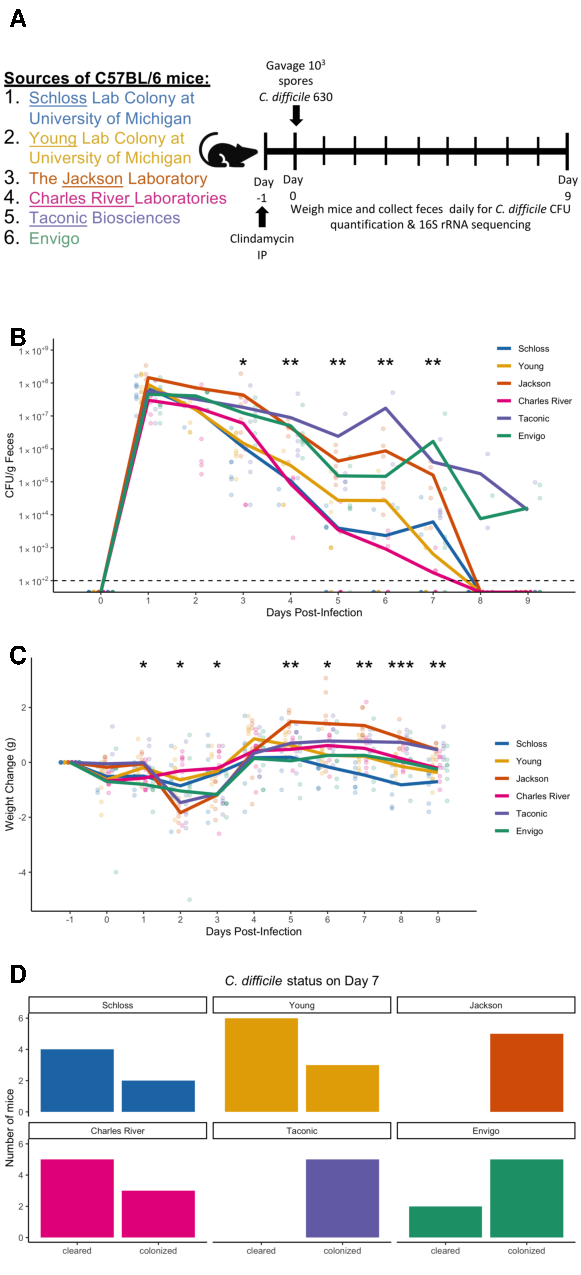
\includegraphics{figure_1.pdf} \textbf{Figure 1. Clindamycin is
sufficient to promote \emph{C. difficile} colonization in all mice, but
clearance time varies across sources of C57BL/6 mice.} A. Setup of the
experimental timeline. Mice for the experiments were obtained from 6
different sources: the Schloss (N = 8) and Young lab (N = 9) colonies at
the University of Michigan, the Jackson Laboratory (N = 8), Charles
River Laboratory (N = 8), Taconic Biosciences (N = 8), and Envigo (N =
8). All mice were administered 10 mg/kg clindamycin intraperitoneally
(IP) 1 day before challenge with \emph{C. difficile} 630 spores on day
0. Mice were weighed and feces was collected daily through the end of
the experiment (9 days post-infection). Note: 3 mice died during course
of experiment. 1 Taconic mouse prior to infection and 1 Jackson and 1
Envigo mouse between 1- and 3-days post-infection. B. \emph{C.
difficile} CFU/gram stool measured over time (N = 20-49 mice per
timepoint) via serial dilutions. The black line represents the limit of
detection for the first serial dilution. CFU quantification data was not
available for each mouse due to early deaths, stool sampling
difficulties, and not plating all of the serial dilutions. C. Mouse
weight change measured in grams over time (N = 45-49 mice per
timepoint), all mice were normalized to the weight recorded 1 day before
infection. For B-C: timepoints where differences across sources of mice
were statistically significant by Kruskal-Wallis test with
Benjamini-Hochberg correction for testing across multiple days (Table S1
and Table S2) are reflected by the asterisk(s) above each timepoint (*,
\emph{P} \textless{} 0.05). Lines represent the median for each source
and circles represent individual mice from experiment 1 while triangles
represent mice from experiment 2. D. \emph{C. difficile} CFU/gram stool
on day 7 post-infection across sources of mice with asterisks for
pairwise Wilcoxon comparisons with Benjamini-Hochberg correction where
\emph{P} \textless{} 0.05. E. Mouse weight change 2 days post-infection
across sources of mice, no pairwise Wilcoxon comparisons were
significant after Benjamini-Hochberg correction. For D-E. Circles
represent experiment 1 mice, triangles represent experiment 2 mice and
gray lines indicate the median values for each group.

\newpage

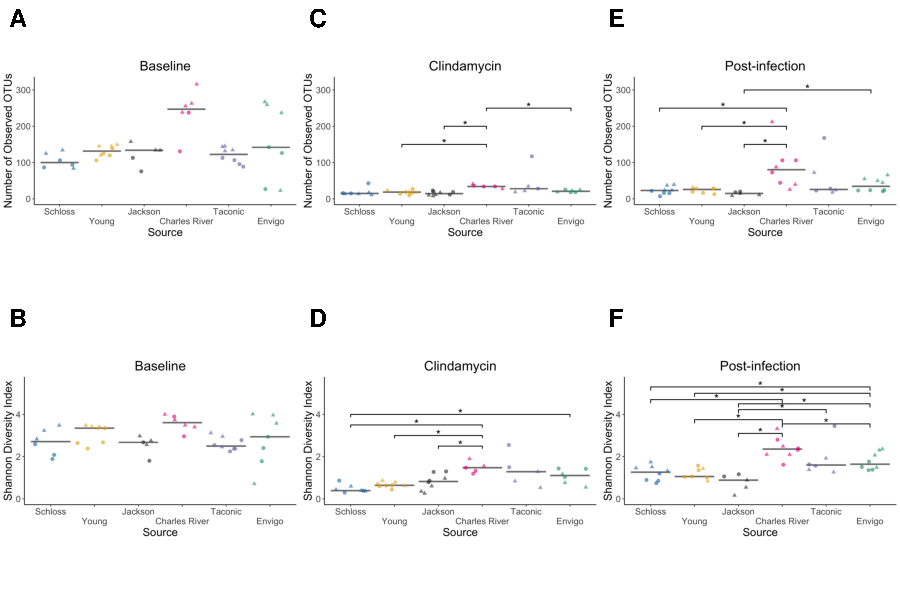
\includegraphics{figure_2.pdf} \textbf{Figure 2. Differences in
microbial richness and diversity across mouse colony sources emerge
after clindamycin treatment and infection.} A-F. Number of observed OTUs
and Shannon diversity index values at baseline: day -1 (A-B), after
clindamycin: day 0 (C-D) and post-infection: day 1 (E-F) timepoints of
the experiment. Data were analyzed by Kruskal-Wallis test with
Benjamini-Hochberg correction for testing each day of the experiment and
the adjusted \emph{P} value was \textless{} 0.05 for all panels except
for B (Table S3). Significant \emph{P} values from the pairwise Wilcoxon
comparisons between sources with Benjamini-Hochberg correction are shown
(Table S4). For A-F: circles represent experiment 1 mice, while
triangles represent experiment 2 mice with each symbol representing the
value for a stool sample from an individual mouse. Gray lines represent
the median values for each source of mice.

\newpage

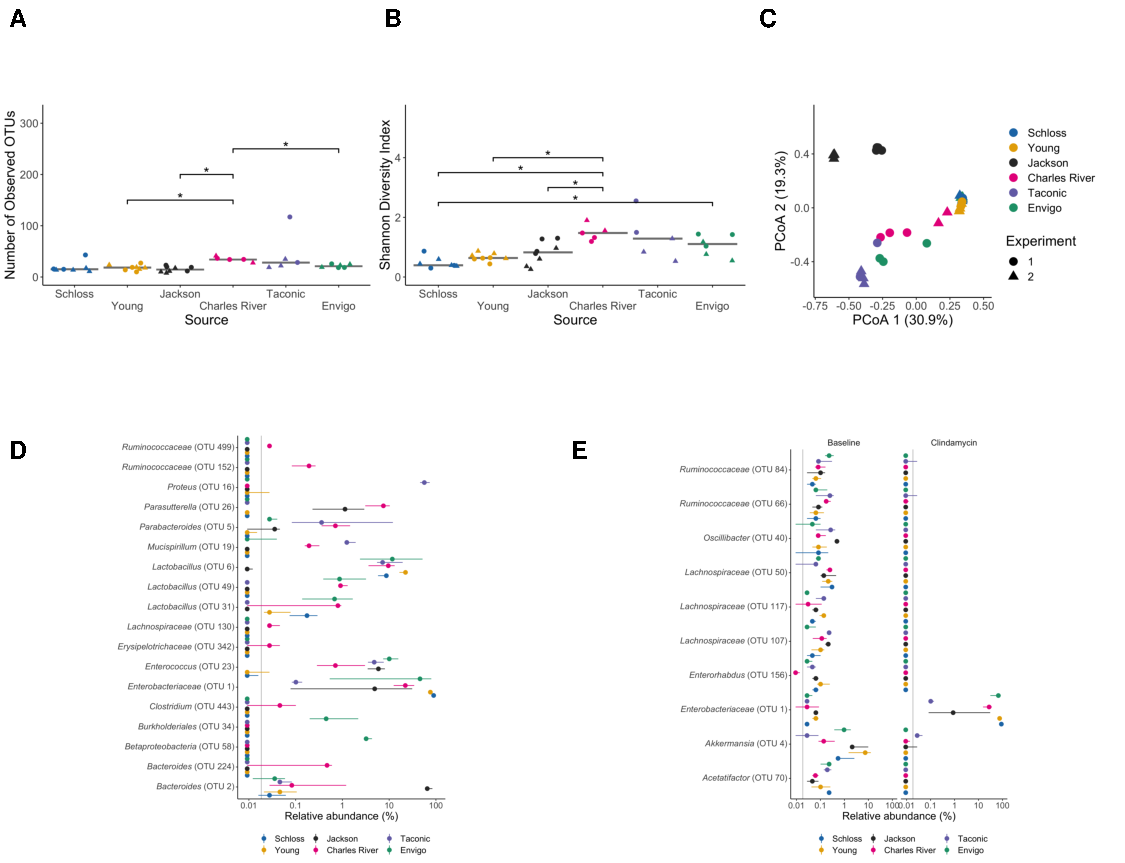
\includegraphics{figure_3.pdf} \textbf{Figure 3. Mouse colony source is
the variable that explains most of the variation observed in the
baseline, post-clindamycin, and post-infection bacterial communities.}
A-C. Principal Coordinates Analysis of Theta YC distances from stools
collected at baseline (A), post-clindamycin (B), and post-infection (C)
timepoints of the experiment. Each symbol represents a stool sample from
an individual mouse, with circles representing experiment 1 mice and
triangles representing experiment 2 mice. PERMANOVA analysis
demonstrated that source and the interaction between source and cage
explained most of the variation observed in the baseline (combined
R\textsuperscript{2} = 0.90), post-clindamycin (combined
R\textsuperscript{2} = 0.99), and post-infection (combined
R\textsuperscript{2} = 0.88) communities (all \emph{P} = 0.0001, see
Table S6).

\newpage

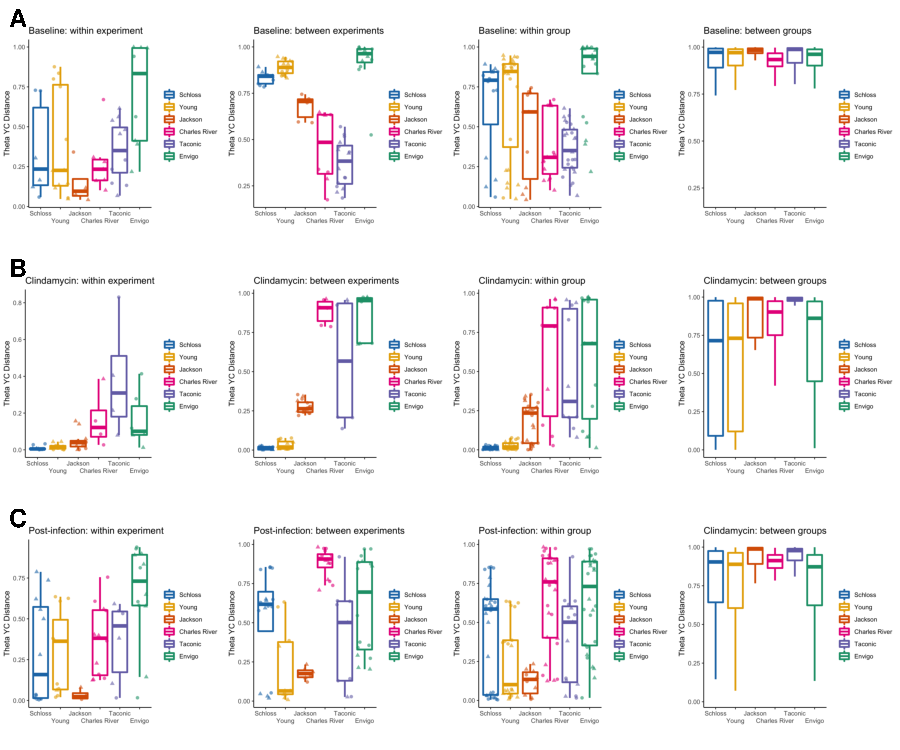
\includegraphics{figure_4.pdf} \textbf{Figure 4. High inter-group
variation across mouse sources is diminished by clindamycin treatment}
A-C. Boxplots of the Theta YC distances of the 6 sources of mice
relative to mice within the same source and experiment, mice within the
same source and between experiments, mice within the same source, and
mice from other groups at the baseline (A), after clindamycin treatment
(B), and post-infection (C) timepoints. For comparisons within mice from
the same source, symbols represent individual mouse samples: circles for
experiment 1 and triangles for experiment 2.

\newpage

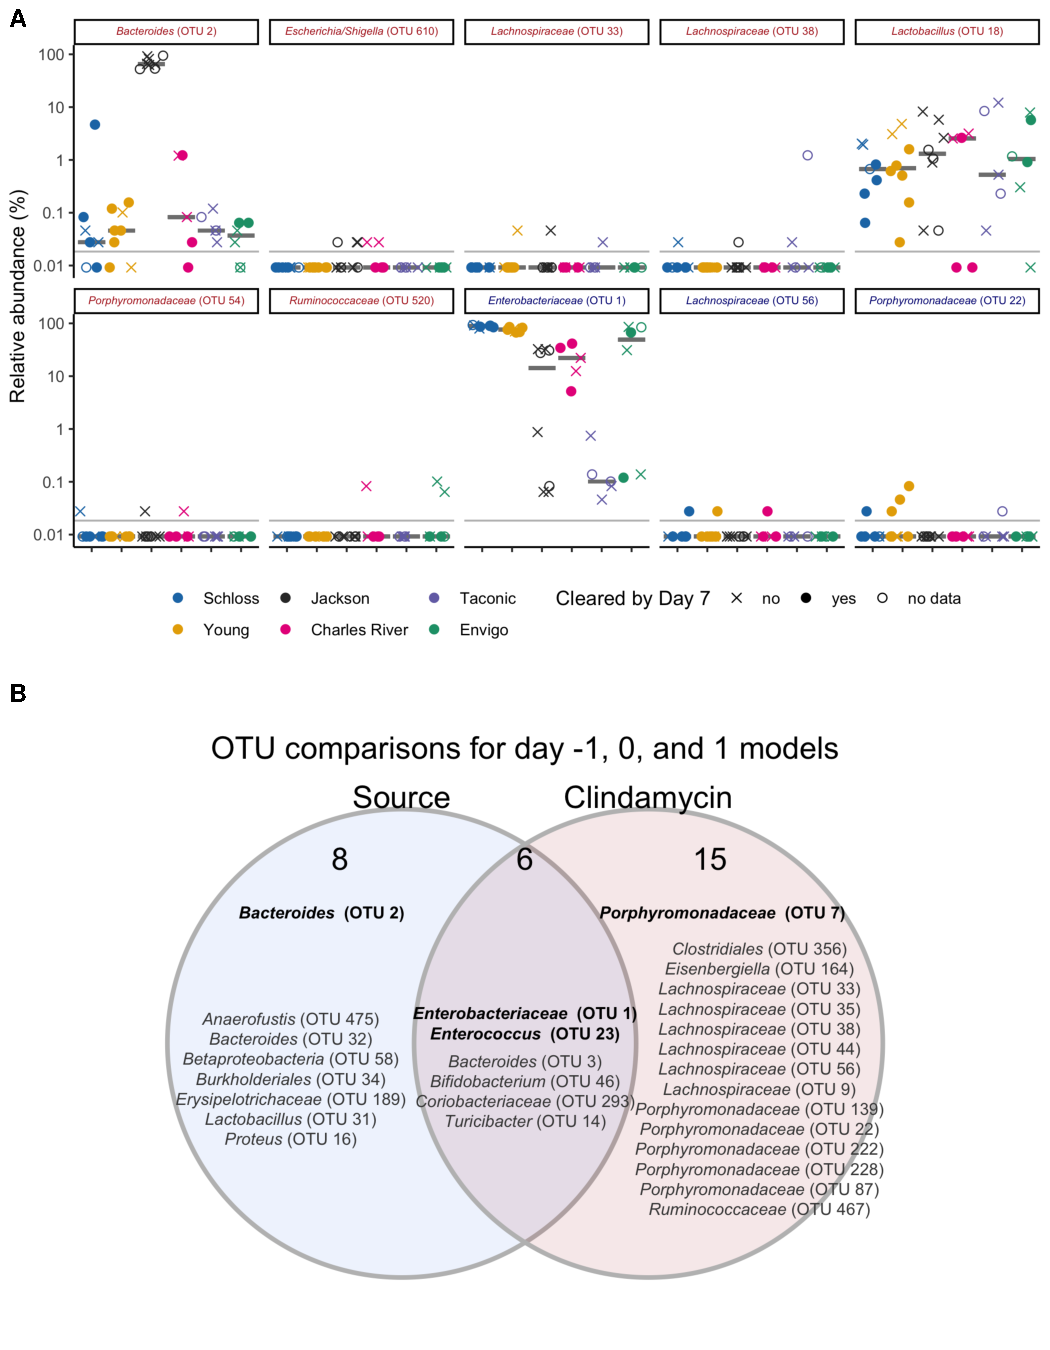
\includegraphics{figure_5.pdf} \textbf{Figure 5. A subset of bacteria
consistently vary across mouse colony sources despite clindamycin
perturbation and \emph{C. difficile} challenge.} A-C. Boxplots of the
relative abundances for the 12 OTUs that consistently varied across
sources of mice at the baseline (A), post-clindamycin (B), and
post-infection (C) timepoints of the experiment. D-F. Boxplots of the
relative abundances for the 8 families that consistently varied across
sources of mice at the baseline (D), post-clindamycin (E), and
post-infection (F) timepoints of the experiment. For each timepoint
bacteria with differential relative abundances across sources of mice
were identified by Kruskal-Wallis test at the family and OTU level with
Benjamini-Hochberg correction for testing all identified taxa at the
respective level (Table S8-9). The grey vertical line indicates the
limit of detection for A-F.

\newpage

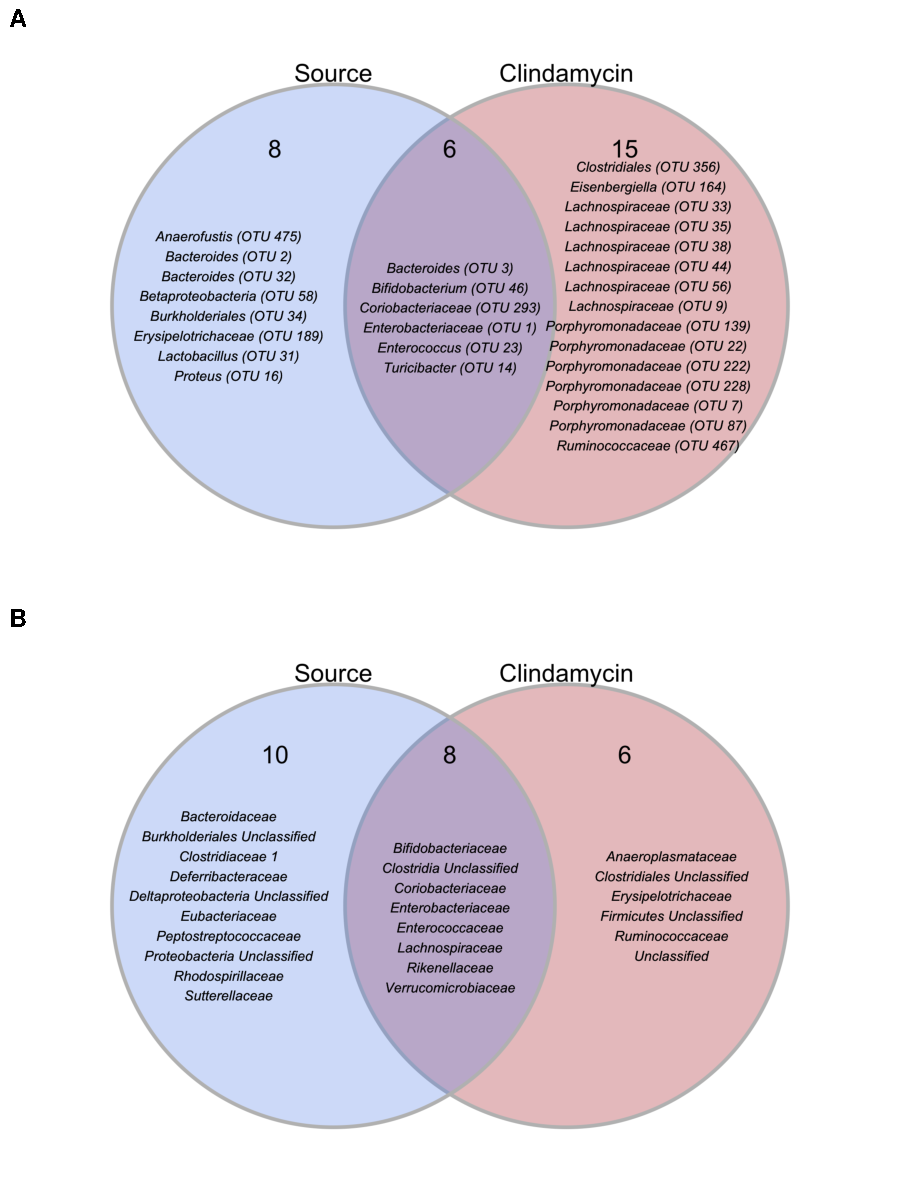
\includegraphics{figure_6.pdf} \textbf{Figure 6. Clindamycin treatment
has the same effects on a subset of taxa regardless of colony source.}
A-B. Boxplots of the top 10 most significant (adjusted \emph{P} value
\textless{} 0.05) OTUs with relative abundances that changed post
clindamycin treatment. C-D. Boxplots of the top 10 most significant
families with relative abundances that changed post clindamycin
treatment. Data were analyzed by Wilcoxon signed rank test limited to
mice that had paired sequence data for day -1 and 0 (N = 31). Tests were
performed at the OTU and family levels with Benjamini-Hochberg
correction for testing all identified OTUs and families. See Table
S10-11 for complete list of OTUs and families significantly impacted by
clindamycin treatment. The grey vertical line indicates the limit of
detection for A-D.

\newpage

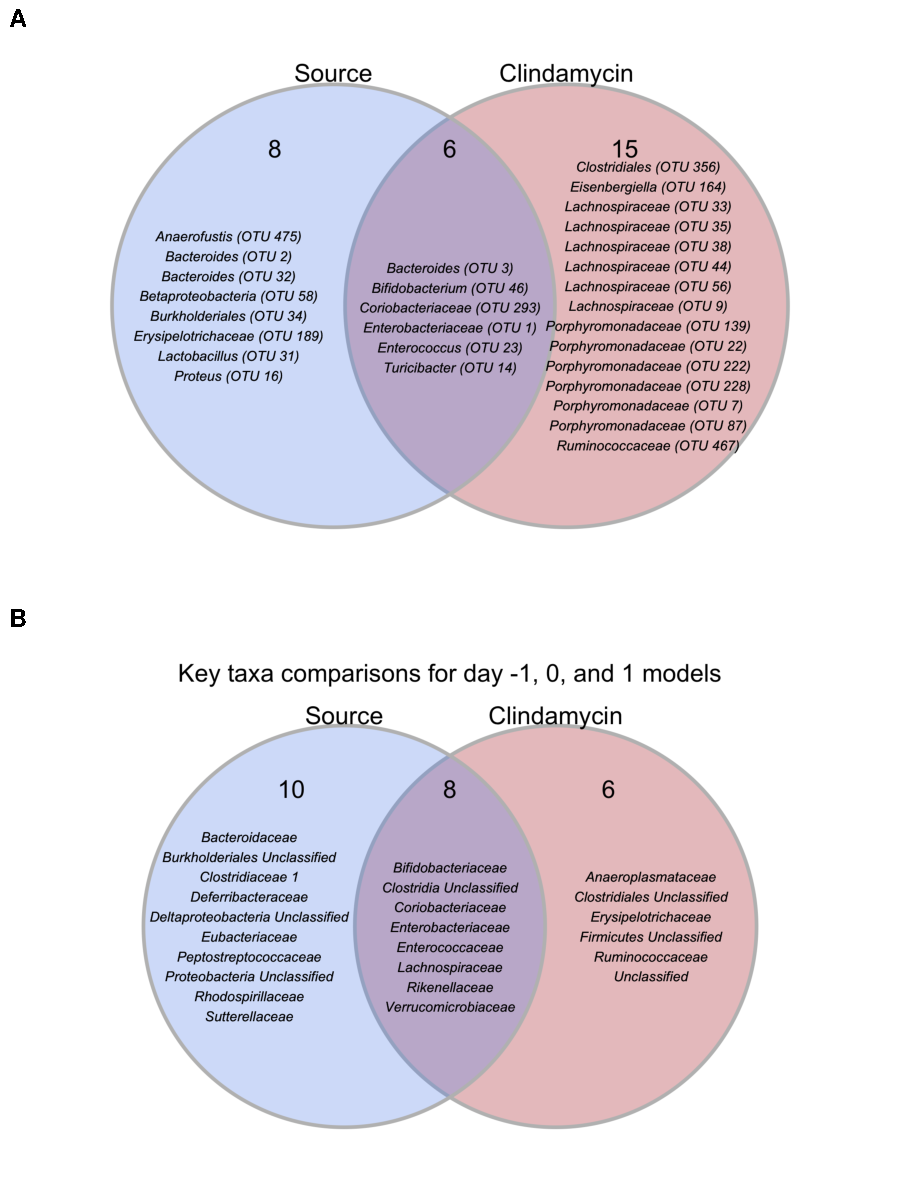
\includegraphics{figure_7.pdf} \textbf{Figure 7. Key OTUs that influence
whether mice cleared \emph{C. difficile} by day 7.} A. Baseline relative
abundance data for 3 of the OTUs from the classification model based on
day 0 OTU relative abundances that significantly varied across sources
of mice and had high relative abundances. Symbols represent the relative
abundance data for an individual mouse, circles represent mice that
cleared \emph{C. difficile} by day 7, X-shapes represent mice that were
still colonized with \emph{C. difficile}, and open circles represent
mice that did not have \emph{C. difficile} CFU counts for day 7
post-infection. Gray lines indicate the median relative abundances for
each source. Asterisks are shown for pairwise Wilcoxon comparisons with
Benjamini-Hochberg correction where \emph{P} \textless{} 0.05. B. Venn
diagram that combines Fig. S4 summaries of OTUs that were important to
the day -1, 0, and 1 classification models (Table S14) and either
overlapped with taxa that varied across vendors at the same timepoint,
were impacted by clindamycin treatment, or both. See Fig. S4 for
separate comparisons of taxa from the day -1, 0, and 1 classification
models. Bold OTUs signify OTUs that were important to more than 1
classification model.

\newpage

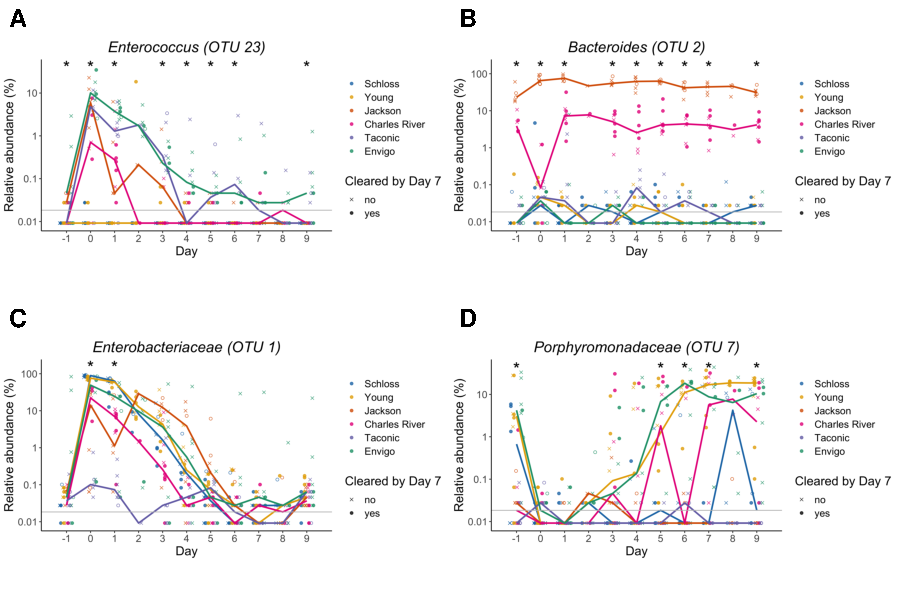
\includegraphics{figure_8.pdf} \textbf{Figure 8: Key OTUs vary across
sources throughout the experiment.} A-C. Relative abundances of bold
OTUs from Fig. 7A that were important for at least two classification
models are shown over time. A. \emph{Enterococcus} (OTU 23), which
significantly varied across sources and was impacted by clindamycin
treatment. B. \emph{Bacteroides} (OTU 2), which varied across sources
throughout the experiment. C. \emph{Enterobacteriaceae} (OTU 1) and
\emph{Porphyromonadaceae} (OTU 7) were significantly impacted by
clindamycin treatment and examining relative abundance dynamics over the
course of the experiment indicated timepoints where relative abundances
also significantly varied across sources of mice. Symbols represent the
relative abundance data for an individual mouse, circles represent mice
that cleared \emph{C. difficile} by day 7, X-shapes represent mice that
were still colonized with \emph{C. difficile}, and open circles
represent mice that did not have \emph{C. difficile} CFU counts for day
7 post-infection. Colored lines indicate the median relative abundances
for each source. The gray horizontal line represents the limit of
detection. Timepoints where differences across sources of mice were
statistically significant by Kruskal-Wallis test with Benjamini-Hochberg
correction for testing across multiple days (Table S16) are identified
by the asterisk(s) above each timepoint (*, P \textless{} 0.05).

\newpage

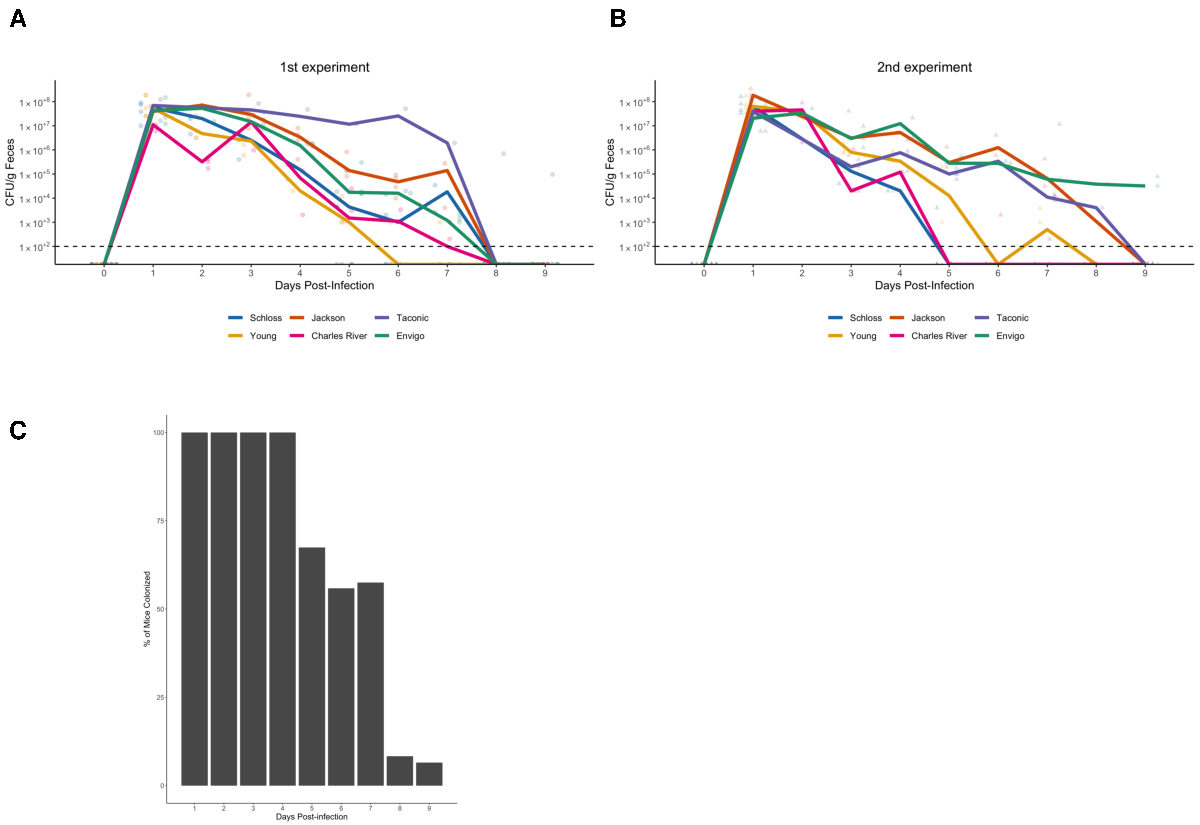
\includegraphics{figure_S1.pdf} \textbf{Figure S1. \emph{C. difficile}
CFU variation across vendors varies slightly across the 2 experiments.}
A-B. \emph{C. difficile} CFU/gram of stool quantification over time for
experiment 1 (A) and 2 (B). Experiments were conducted approximately 3
months apart. Lines represent the median CFU for each source, symbols
represent individual mice and the black line represents the limit of
detection. C. Percent of mice that were colonized with \emph{C.
difficile} over the course of the experiment. Each day the percent is
calculated based on the mice where \emph{C. difficile} CFU was
quantified for that particular day. Total N for each day: day 1 (N =
42), day 2 (N = 20), day 3 (N = 39), day 4 (N = 29), day 5 (N = 43), day
6 (N = 34), day 7 (N = 40), day 8 (N = 36), and day 9 (N = 46).

\newpage

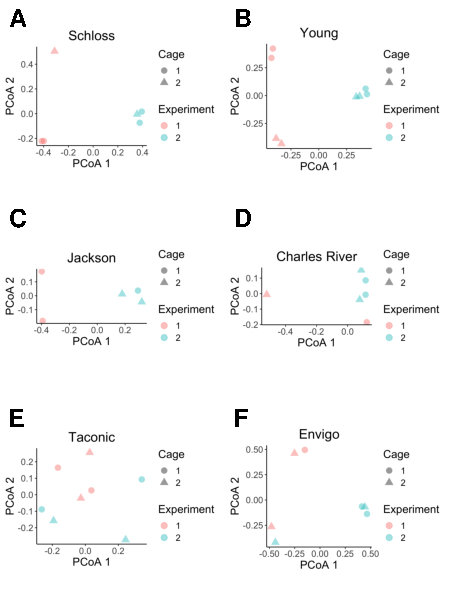
\includegraphics{figure_S2.pdf} \textbf{Figure S2. Only bacterial
communities from University of Michigan mice significantly vary between
experiments.} A-F. PCoA of Theta YC distances for the baseline fecal
bacterial communities within each source of mice. Each symbol represents
a stool sample from an individual mouse with color corresponding to
experiment and shape representing cage mates. PERMANOVA was performed
within each group to examine the contributions of experiment and cage to
observed variation. Experiment number and cage only significantly
explained observed variation for mice from the Schloss (combined
R\textsuperscript{2} = 0.99; \emph{P} \(\le\) 0.033) and Young (combined
R\textsuperscript{2} = 0.95; \emph{P} \(\le\) 0.027) lab colonies (Table
S7).

\newpage

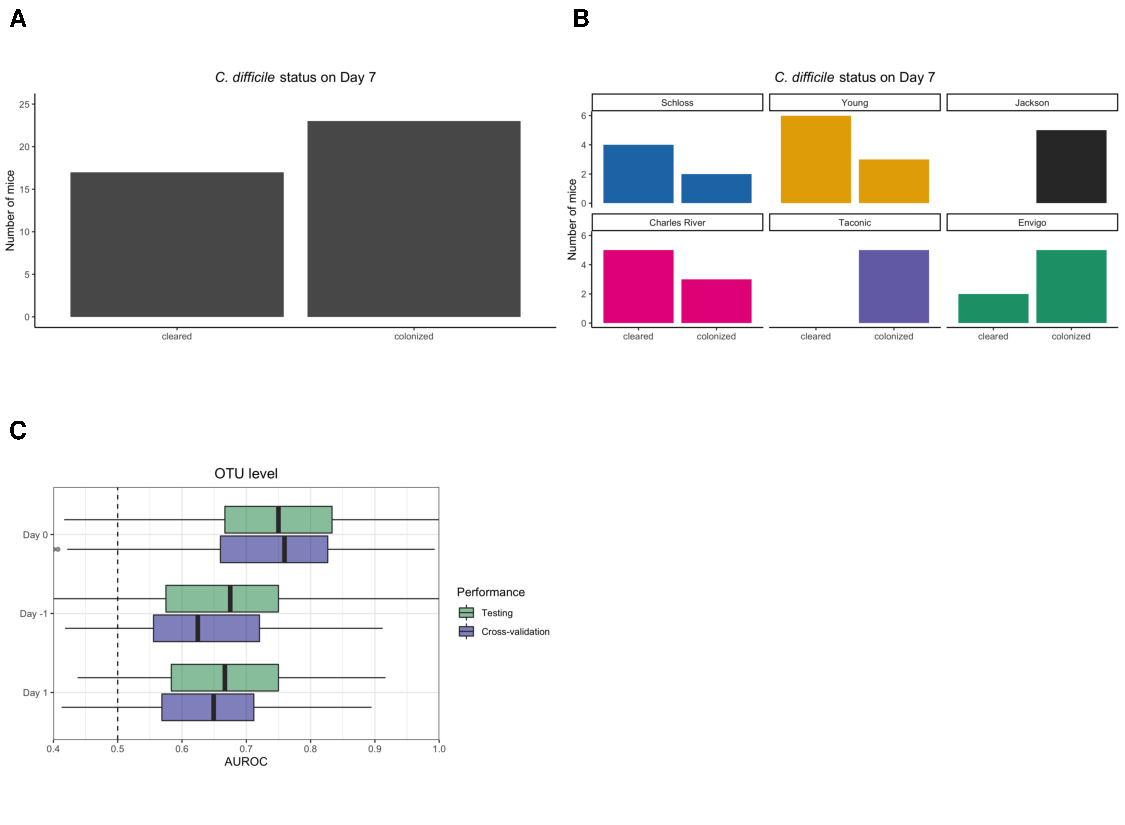
\includegraphics{figure_S3.pdf} \textbf{Figure S3. Bacterial community
composition before, after clindamycin perturbation, and post-infection
can predict \emph{C. difficile} colonization status 7 days
post-challenge.} A. Bar graph visualizations of overall day 7 C.
difficile colonization status that were used as classification outcomes
to build logistic regression models. Mice were classified as colonized
or cleared (not detectable at the limit of detection of 100 CFU) based
on CFU g/stool data from 7 days post-infection. B. \emph{C. difficile}
CFU status on Day 7 within each mouse colony source. N = 5-9 mice per
group. C-D. L2-regularized logistic regression classification model
AUROCs to predict \emph{C. difficile} CFU on D7 (Fig. 1D, Fig. S3) based
on the community relative abundances at baseline (day -1),
post-clindamycin (day 0), and post-infection (day 1) at either the OTU
(C) or family (D) level. All models performed better than random chance
(AUROC = 0.5), see (all \emph{P} \(\le\) 5e-15; Table S12) and the model
built with post-clindamycin treated bacterial OTU relative abundances
had the best performance ((\emph{P}\textsubscript{FDR} \(\le\) 3.9e-10
for pairwise comparisons; Table S13). A List of the 20 taxa that were
ranked as most important to each model are listed in Table S14-15.

\newpage

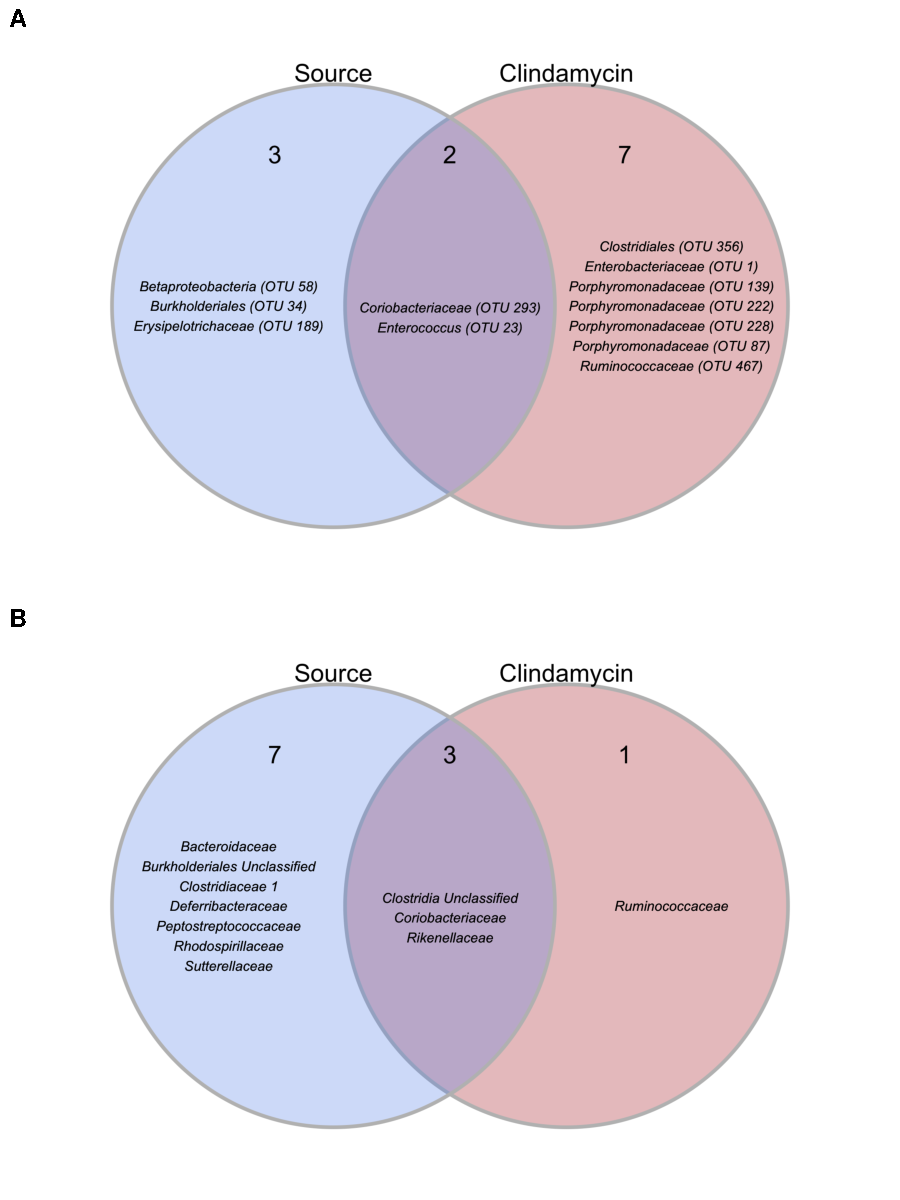
\includegraphics{figure_S4.pdf} \textbf{Figure S4. Key OTUs from
classification models based on baseline, post-clindamycin treatment, or
post-infection community data vary by mouse colony source, clindamycin
treatment, or both.} A-C. Venn diagrams of top 20 important OTUs from
baseline (A), post-clindamycin treatment (B), and post-infection (C)
classification models (Table S14) that overlapped with OTUs that varied
across vendors at baseline, were impacted by clindamycin treatment, or
both. Bold OTUs signify OTUs that were important to more than 1
classification model.

\newpage

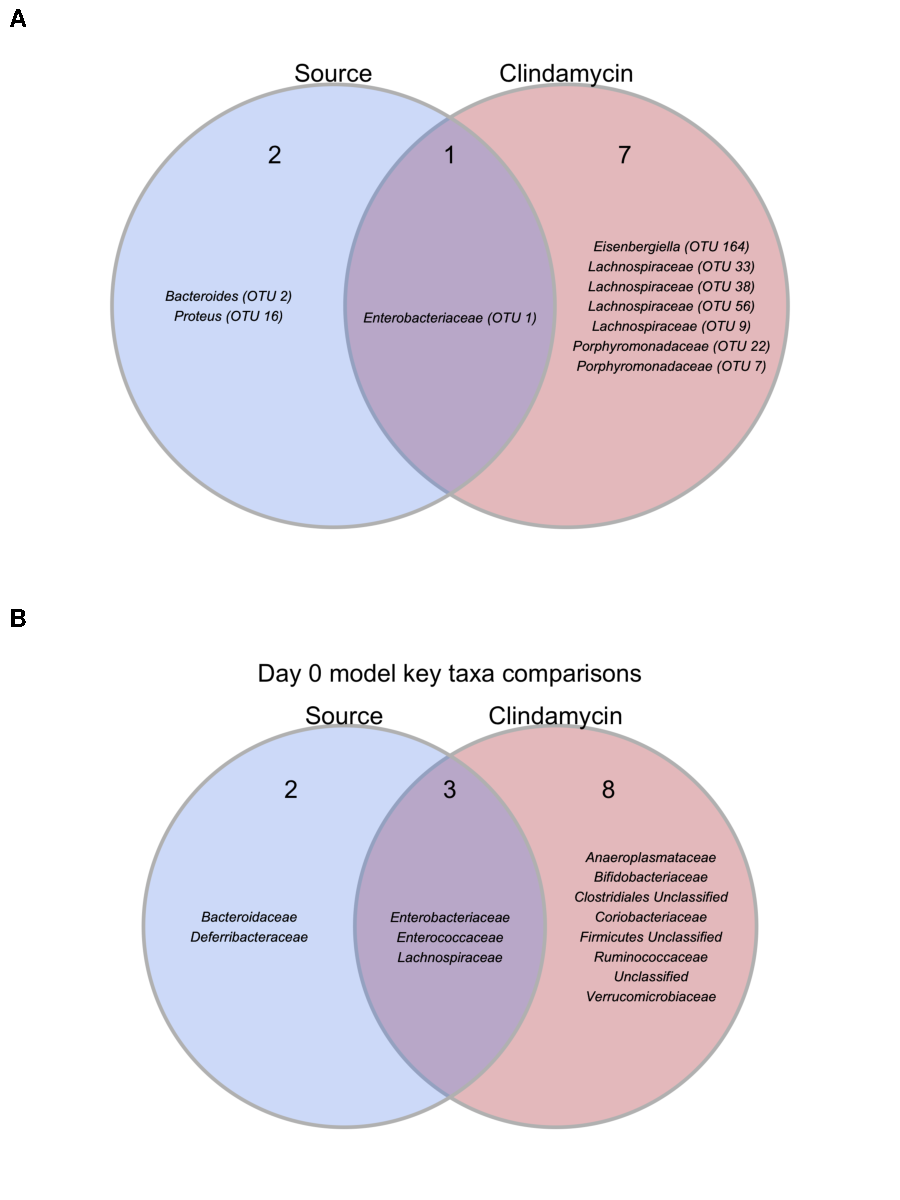
\includegraphics{figure_S5.pdf} \textbf{Figure S5. Key families from
classification models based on baseline, post-clindamycin treatment, or
post-infection community data vary by mouse colony source, clindamycin
treatment, or both.} A-C. Venn diagrams of top 20 important families
from baseline (A), post-clindamycin treatment (B), and post-infection
(C) classification models (Table S15) that overlapped with families that
varied across vendors after clindamycin, were impacted by clindamycin
treatment, or both. D. Venn diagrams that combines A-C summaries of
familes that were important to the day -1, 0, and 1 classification
models (Table S15) and either overlapped with familes that varied across
vendors at the same timepoint, were impacted by clindamycin treatment,
or both. Bold families signify families that were important to more than
1 classification model.

\newpage

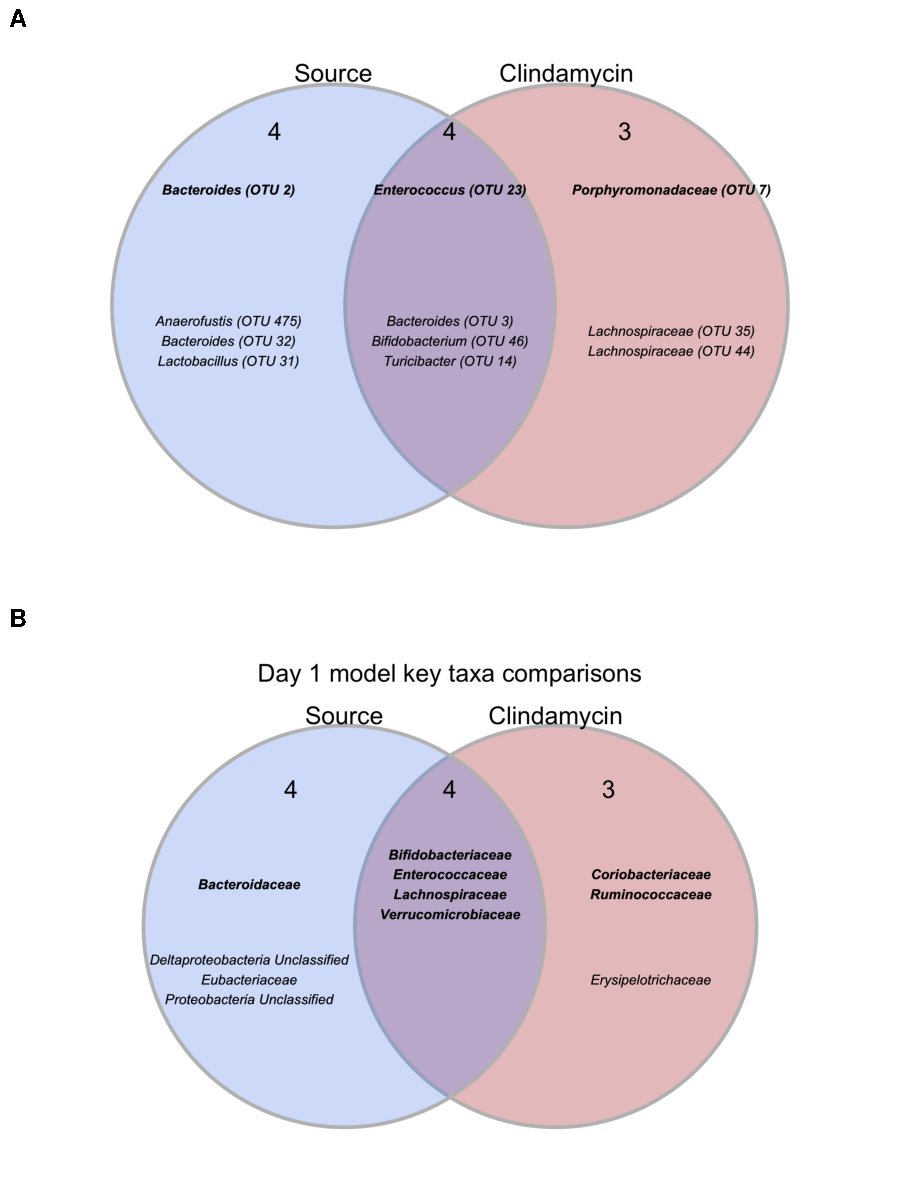
\includegraphics{figure_S6.pdf} \textbf{Figure S6. Key families vary
across sources throughout experiment.} Relative abundances of bold
families from Fig. S5D that were important for at least two
classification models are shown over time. A. \emph{Enterococcaceae} and
\emph{Lachnospiraceae}, which significantly varied across sources and
were impacted by clindamycin treatment. B. \emph{Bacteroidaceae} and
\emph{Deferribacteraceae}, which varied across sources throughout the
experiment. C. \emph{Bifidobacteriaceae}, \emph{Coriobacteriaceae},
\emph{Ruminococcaceae}, and \emph{Verrucomicrobiaceae} were
significantly impacted by clindamycin treatment. Examining the relative
abundance dynamics throughout the experiment, identified timepoints
where relative abundances also significantly varied across sources of
mice. Symbols represent the relative abundance data for an individual
mouse, circles represent mice that cleared \emph{C. difficile} by day 7,
X-shapes represent mice that were still colonized with \emph{C.
difficile}, and open circles represent mice that did not have \emph{C.
difficile} CFU counts for day 7 post-infection. Colored lines indicate
the median relative abundances for each source. The gray horizontal line
represents the limit of detection. Timepoints where differences across
sources of mice were statistically significant by Kruskal-Wallis test
with Benjamini-Hochberg correction for testing across multiple days
(Table S17) are identified by the asterisk(s) above each timepoint (*, P
\textless{} 0.05).

\newpage

\subsection{Supplementary Tables and
Movie}\label{supplementary-tables-and-movie}

All supplemental material is available at:
\url{https://github.com/SchlossLab/Tomkovich_vendor_difs_XXXX_2020/submission}.

\textbf{Movie S1. Large shifts in bacterial community structure occurred
after clindamycin and \emph{C. difficile} infection.} PCoA of Theta YC
distances animated from 0 through 9 days post-infection. PERMANOVA
analysis indicated colony source was the variable that explained the
most observed variation across fecal communities (source
R\textsuperscript{2} = 0.35, \emph{P} = 0.0001) followed by interactions
between cage and day of the experiment. Transparency of the circle
corresponds to the day of the experiment, each circle represents a
sample from an individual mouse at a specific timepoint. See Table S5
for PERMANOVA results). Circles represent mice from experiment 1 and
triangles represent mice from expeirment 2.

\textbf{Table S1. \emph{C. difficile} CFU statistical results.}

\textbf{Table S2. Mouse weight change statistical results.}

\textbf{Table S3. Diversity metrics Kruskal-Wallis statistical results.}

\textbf{Table S4. Diversity metrics pairwise Wilcoxon statistical
results.}

\textbf{Table S5. PERMANOVA results for all mice, all timepoints.}

\textbf{Table S6. PERMANOVA results for all mice, all timepoints.}

\textbf{Table S7. PERMANOVA results of baseline communities within each
source.}

\textbf{Table S8. OTUs with relative abudances that significantly vary
across sources at baseline, post-clindamycin, or post-infection
timepoints.}

\textbf{Table S9. Families with relative abudances that significantly
vary across sources at baseline, post-clindamycin, or post-infection
timepoints.}

\textbf{Table S10. OTUs with relative abudances that significantly
changed after clindamycin treatment.}

\textbf{Table S11. Families with relative abudances that significantly
changed after clindamycin treatment.} \textbf{Table S12. Statistical
results of L2-regularized logistic regression model performances
compared to random chance.}

\textbf{Table S13. Pairwise Wilcoxan results of comparing all 6
L2-regularized logistic regression model performances.}

\textbf{Table S14. Top 20 most important OTUs for each of the 3
L2-regularized logistic regression models based on OTU relative
abundance data.}

\textbf{Table S15. Top 20 most important families for each of the 3
L2-regularized logistic regression models based on OTU relative
abundance data.}

\textbf{Table S16. OTUs with relative abudances that significantly
varied across sources of mice on at least 1 day of the experiment.}

\textbf{Table S17. Families with relative abudances that significantly
varied across sources of mice on at least 1 day of the experiment.}


\end{document}
